% Options for packages loaded elsewhere
\PassOptionsToPackage{unicode}{hyperref}
\PassOptionsToPackage{hyphens}{url}
%
\documentclass[
  ignorenonframetext,
  aspectratio=169]{beamer}
\usepackage{pgfpages}
\setbeamertemplate{caption}[numbered]
\setbeamertemplate{caption label separator}{: }
\setbeamercolor{caption name}{fg=normal text.fg}
\beamertemplatenavigationsymbolsempty
% Prevent slide breaks in the middle of a paragraph
\widowpenalties 1 10000
\raggedbottom
\setbeamertemplate{part page}{
  \centering
  \begin{beamercolorbox}[sep=16pt,center]{part title}
    \usebeamerfont{part title}\insertpart\par
  \end{beamercolorbox}
}
\setbeamertemplate{section page}{
  \centering
  \begin{beamercolorbox}[sep=12pt,center]{part title}
    \usebeamerfont{section title}\insertsection\par
  \end{beamercolorbox}
}
\setbeamertemplate{subsection page}{
  \centering
  \begin{beamercolorbox}[sep=8pt,center]{part title}
    \usebeamerfont{subsection title}\insertsubsection\par
  \end{beamercolorbox}
}
\AtBeginPart{
  \frame{\partpage}
}
\AtBeginSection{
  \ifbibliography
  \else
    \frame{\sectionpage}
  \fi
}
\AtBeginSubsection{
  \frame{\subsectionpage}
}
\usepackage{amsmath,amssymb}
\usepackage{lmodern}
\usepackage{iftex}
\ifPDFTeX
  \usepackage[T1]{fontenc}
  \usepackage[utf8]{inputenc}
  \usepackage{textcomp} % provide euro and other symbols
\else % if luatex or xetex
  \usepackage{unicode-math}
  \defaultfontfeatures{Scale=MatchLowercase}
  \defaultfontfeatures[\rmfamily]{Ligatures=TeX,Scale=1}
\fi
\usecolortheme{orchid}
% Use upquote if available, for straight quotes in verbatim environments
\IfFileExists{upquote.sty}{\usepackage{upquote}}{}
\IfFileExists{microtype.sty}{% use microtype if available
  \usepackage[]{microtype}
  \UseMicrotypeSet[protrusion]{basicmath} % disable protrusion for tt fonts
}{}
\makeatletter
\@ifundefined{KOMAClassName}{% if non-KOMA class
  \IfFileExists{parskip.sty}{%
    \usepackage{parskip}
  }{% else
    \setlength{\parindent}{0pt}
    \setlength{\parskip}{6pt plus 2pt minus 1pt}}
}{% if KOMA class
  \KOMAoptions{parskip=half}}
\makeatother
\usepackage{xcolor}
\IfFileExists{xurl.sty}{\usepackage{xurl}}{} % add URL line breaks if available
\IfFileExists{bookmark.sty}{\usepackage{bookmark}}{\usepackage{hyperref}}
\hypersetup{
  pdftitle={Supervised Learning II: high-dimensional model selection},
  hidelinks,
  pdfcreator={LaTeX via pandoc}}
\urlstyle{same} % disable monospaced font for URLs
\newif\ifbibliography
\usepackage{color}
\usepackage{fancyvrb}
\newcommand{\VerbBar}{|}
\newcommand{\VERB}{\Verb[commandchars=\\\{\}]}
\DefineVerbatimEnvironment{Highlighting}{Verbatim}{commandchars=\\\{\}}
% Add ',fontsize=\small' for more characters per line
\usepackage{framed}
\definecolor{shadecolor}{RGB}{248,248,248}
\newenvironment{Shaded}{\begin{snugshade}}{\end{snugshade}}
\newcommand{\AlertTok}[1]{\textcolor[rgb]{0.94,0.16,0.16}{#1}}
\newcommand{\AnnotationTok}[1]{\textcolor[rgb]{0.56,0.35,0.01}{\textbf{\textit{#1}}}}
\newcommand{\AttributeTok}[1]{\textcolor[rgb]{0.77,0.63,0.00}{#1}}
\newcommand{\BaseNTok}[1]{\textcolor[rgb]{0.00,0.00,0.81}{#1}}
\newcommand{\BuiltInTok}[1]{#1}
\newcommand{\CharTok}[1]{\textcolor[rgb]{0.31,0.60,0.02}{#1}}
\newcommand{\CommentTok}[1]{\textcolor[rgb]{0.56,0.35,0.01}{\textit{#1}}}
\newcommand{\CommentVarTok}[1]{\textcolor[rgb]{0.56,0.35,0.01}{\textbf{\textit{#1}}}}
\newcommand{\ConstantTok}[1]{\textcolor[rgb]{0.00,0.00,0.00}{#1}}
\newcommand{\ControlFlowTok}[1]{\textcolor[rgb]{0.13,0.29,0.53}{\textbf{#1}}}
\newcommand{\DataTypeTok}[1]{\textcolor[rgb]{0.13,0.29,0.53}{#1}}
\newcommand{\DecValTok}[1]{\textcolor[rgb]{0.00,0.00,0.81}{#1}}
\newcommand{\DocumentationTok}[1]{\textcolor[rgb]{0.56,0.35,0.01}{\textbf{\textit{#1}}}}
\newcommand{\ErrorTok}[1]{\textcolor[rgb]{0.64,0.00,0.00}{\textbf{#1}}}
\newcommand{\ExtensionTok}[1]{#1}
\newcommand{\FloatTok}[1]{\textcolor[rgb]{0.00,0.00,0.81}{#1}}
\newcommand{\FunctionTok}[1]{\textcolor[rgb]{0.00,0.00,0.00}{#1}}
\newcommand{\ImportTok}[1]{#1}
\newcommand{\InformationTok}[1]{\textcolor[rgb]{0.56,0.35,0.01}{\textbf{\textit{#1}}}}
\newcommand{\KeywordTok}[1]{\textcolor[rgb]{0.13,0.29,0.53}{\textbf{#1}}}
\newcommand{\NormalTok}[1]{#1}
\newcommand{\OperatorTok}[1]{\textcolor[rgb]{0.81,0.36,0.00}{\textbf{#1}}}
\newcommand{\OtherTok}[1]{\textcolor[rgb]{0.56,0.35,0.01}{#1}}
\newcommand{\PreprocessorTok}[1]{\textcolor[rgb]{0.56,0.35,0.01}{\textit{#1}}}
\newcommand{\RegionMarkerTok}[1]{#1}
\newcommand{\SpecialCharTok}[1]{\textcolor[rgb]{0.00,0.00,0.00}{#1}}
\newcommand{\SpecialStringTok}[1]{\textcolor[rgb]{0.31,0.60,0.02}{#1}}
\newcommand{\StringTok}[1]{\textcolor[rgb]{0.31,0.60,0.02}{#1}}
\newcommand{\VariableTok}[1]{\textcolor[rgb]{0.00,0.00,0.00}{#1}}
\newcommand{\VerbatimStringTok}[1]{\textcolor[rgb]{0.31,0.60,0.02}{#1}}
\newcommand{\WarningTok}[1]{\textcolor[rgb]{0.56,0.35,0.01}{\textbf{\textit{#1}}}}
\usepackage{longtable,booktabs,array}
\usepackage{calc} % for calculating minipage widths
\usepackage{caption}
% Make caption package work with longtable
\makeatletter
\def\fnum@table{\tablename~\thetable}
\makeatother
\setlength{\emergencystretch}{3em} % prevent overfull lines
\providecommand{\tightlist}{%
  \setlength{\itemsep}{0pt}\setlength{\parskip}{0pt}}
\setcounter{secnumdepth}{-\maxdimen} % remove section numbering
\AtBeginSection[]{\begin{frame}\frametitle{Today's lecture}\tableofcontents[currentsection]\end{frame}}
\makeatletter
\def\ps@titlepage{%
  \setbeamertemplate{footline}{}
}
\addtobeamertemplate{title page}{\thispagestyle{titlepage}}{}
\makeatother
\include{toc}
\ifLuaTeX
  \usepackage{selnolig}  % disable illegal ligatures
\fi

\title{Supervised Learning II: high-dimensional model selection}
\author{Yongjin Park\\
University of British Columbia}
\date{06 March, 2022}

\begin{document}
\frame{\titlepage}

\begin{frame}{Learning Objectives}
\protect\hypertarget{learning-objectives}{}
\large

\begin{itemize}
\item
  Model selection, Bias-Variance tradeoff, a Bayesian View
\item
  How do we handle \(p \gg n\) situation in practice?
\item
  Multiple Frequenist \& Bayesian approaches
\end{itemize}
\end{frame}

\begin{frame}{A working example: predicting gene expressions from
genetic information}
\protect\hypertarget{a-working-example-predicting-gene-expressions-from-genetic-information}{}
\Large

Q. Can we predict gene expressions based on genetic information?

\centering

DNA \(\overset{\textsf{\color{red} here?}}{\to}\) mRNA \(\to\) protein
\end{frame}

\begin{frame}{If we could predict gene expression\ldots{}}
\protect\hypertarget{if-we-could-predict-gene-expression}{}
\Large

\[\textsf{DNA} \overset{\textsf{\color{red} here?}}{\to} \textsf{mRNA} \to \textsf{protein}\]

\normalsize

We can guess potential mechanisms of genetic disorders:

\Large

\[\textsf{DNA change} \to \overset{\textsf{\color{red} black-box}}{(\cdots)} \to \textsf{disease}\]

\normalsize

because we can do transcriptome-wide association studies (TWAS):

\Large

\[\Delta\textsf{DNA} \to \textsf{mRNA}(\Delta \textsf{DNA}) \overset{\textsf{\color{red} test this}}{\to} \textsf{disease}\]

\tiny Gamazon \emph{et al.} Nature Genetics (2015)

\tiny Gusev \emph{et al.} Nature Genetics (2016)
\end{frame}

\begin{frame}{If we could predict gene expression by genetic
information\ldots{}}
\protect\hypertarget{if-we-could-predict-gene-expression-by-genetic-information}{}
\begin{columns}[T]
\begin{column}{.45\textwidth}
\scriptsize

\onslide<1->{


\begin{center}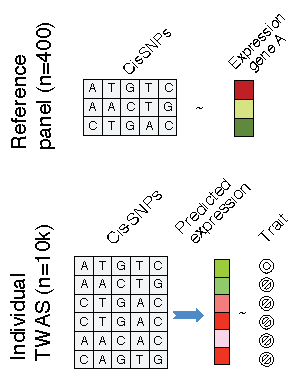
\includegraphics[height=.7\textheight]{Vis/TWAS} \end{center}


}

\normalsize

\tiny Gusev \emph{et al.} Nature Genetics (2016)
\end{column}

\begin{column}{.45\textwidth}
\scriptsize

\onslide<2>{


\begin{center}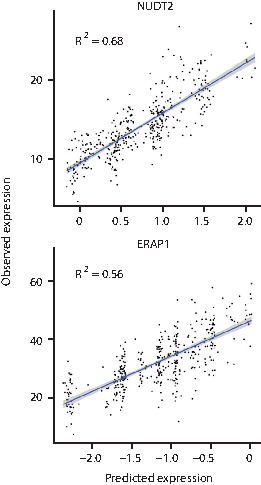
\includegraphics[height=.7\textheight]{Vis/TWAS2} \end{center}


}

\normalsize

\tiny Gamazon \emph{et al.} Nature Genetics (2015)
\end{column}
\end{columns}
\end{frame}

\begin{frame}{Today's problem: gene expression prediction}
\protect\hypertarget{todays-problem-gene-expression-prediction}{}
\Large

\begin{itemize}
\item
  We will focus on supervised learning (regression) of gene expression
\item
  We will revisit the problem in depth in the GWAS and advnaced GWAS
  lectures
\end{itemize}
\end{frame}

\begin{frame}{Why regression?}
\protect\hypertarget{why-regression}{}
\scriptsize

\onslide<1>{


\begin{center}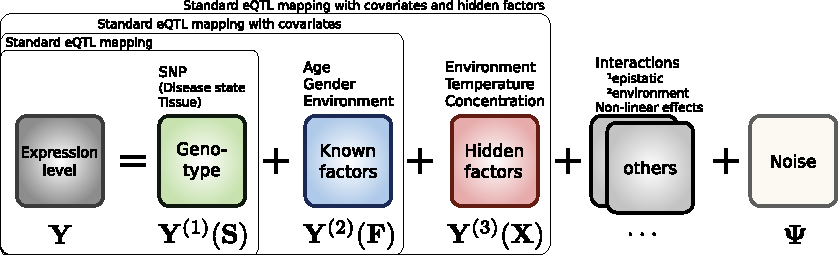
\includegraphics[width=.8\textwidth]{Vis/peer} \end{center}


}

\normalsize

\begin{itemize}
\item
  Handle multiple types of biological and technical factors
\item
  Including all the variables often improve statistical powers
\item
  What if there are too many variables?
\end{itemize}

\vfill

\flushleft{\tiny Stegle {\it et al.} PLoS Genetics (2010)}
\end{frame}

\begin{frame}{Modeling gene expression as a function of genetic
variants}
\protect\hypertarget{modeling-gene-expression-as-a-function-of-genetic-variants}{}
\[
\mathbf{y} = \left(\begin{array}{l}
y_{1}\\
y_{2}\\
\vdots\\
y_{n}
\end{array}\right),\quad
X = \left(\begin{array}{l l l}
X_{11} & \cdots & X_{1p} \\
X_{21} & \cdots & X_{2p} \\
 & \cdots & \\
X_{n1} & \cdots & X_{np} \\
\end{array}\right),\quad
\boldsymbol{\theta} = \left(\begin{array}{l}
\theta_{1}\\
\theta_{2}\\
\vdots\\
\theta_{p}
\end{array}\right)
\]

\vfill

\textbf{Multivariate linear regression model:} \[
\mathbf{y} = X \boldsymbol{\theta} + \epsilon,\, \boldsymbol{\epsilon} \sim \mathcal{N}\!\left(\mathbf{0}, \sigma^{2}I\right).
\]

\vfill

\textbf{Example}

\begin{itemize}
\item
  \(\mathbf{y}\) : a gene expression measured by RNA-seq / microarray.
\item
  \({(X_{ij})}\) : genetic variants at locus \(j\) measured on
  individual \(i\). \(X\) can be anything of interest, such as other
  genes and phenotypes.
\item
  We can fit the model gene by gene (independence) or all the genes
  jointly (dependency between genes)
\end{itemize}
\end{frame}

\begin{frame}{Two major interests in regression analysis}
\protect\hypertarget{two-major-interests-in-regression-analysis}{}
\[
\mathbf{y} = \left(\begin{array}{l}
y_{1}\\
y_{2}\\
\vdots\\
y_{n}
\end{array}\right),\quad
X = \left(\begin{array}{l l l}
X_{11} & \cdots & X_{1p} \\
X_{21} & \cdots & X_{2p} \\
 & \cdots & \\
X_{n1} & \cdots & X_{np} \\
\end{array}\right),\quad
\boldsymbol{\theta} = \left(\begin{array}{l}
\theta_{1}\\
\theta_{2}\\
\vdots\\
\theta_{p}
\end{array}\right)
\]

\vfill

\emph{Multivariate linear regression model:} \[
\mathbf{y} = X \boldsymbol{\theta} + \epsilon,\, \boldsymbol{\epsilon} \sim \mathcal{N}\!\left(\mathbf{0}, \sigma^{2}I\right).
\]

\vfill

\onslide<2->{
1. Estimation of unknown parameters (\textbf{posterior probability}):
$$
p(\boldsymbol{\theta}|X,\mathbf{y}) \propto p(\mathbf{y}|X,\boldsymbol{\theta}) p(\boldsymbol{\theta})
$$
}

\onslide<3->{
2. Prediction of future phenotype (\textbf{posterior prediction}):
$$
p(\mathbf{y}^{\textrm{new}}|X^{\textrm{new}},X,\mathbf{y}) = \int p(\mathbf{y}^{\textrm{new}}|X^{\textrm{new}},\boldsymbol{\theta}) p(\mathbf{y}|X,\boldsymbol{\theta}) p(\boldsymbol{\theta}) d\boldsymbol{\theta}
$$
}
\end{frame}

\begin{frame}{Reconciling two related concepts -- MLE and MSE}
\protect\hypertarget{reconciling-two-related-concepts-mle-and-mse}{}
Equivalence of maximum-likelihood estimation and mean square error
minimization (isotropic Gaussian error distribution).

\vfill

\textbf{{[}MLE{]}} Find \({\boldsymbol{\theta}}\) maximizing \[
\ln p(\mathbf{y}|X,\boldsymbol{\theta})
= - \frac{1}{2\sigma^{2}} \sum_{i=1}^{n} (y_{i} - \mathbf{x}_{i} \boldsymbol{\theta})^{2} + \textrm{const.}
\] \emph{without prior contribution of parameter, and \(\sigma\) is
known.}

\vfill

\textbf{{[}MSE{]}} Find \(\boldsymbol{\theta}\) minimizing \[
\sum_{i=1}^{n} (y_{i} - \mathbf{x}_{i} \boldsymbol{\theta})^{2}.
\]

\vfill
\end{frame}

\begin{frame}{MLE, MSE, an optimization problem}
\protect\hypertarget{mle-mse-an-optimization-problem}{}
Minimization of the convex loss function: \[
L(\boldsymbol{\theta}) = (\mathbf{y} - X\boldsymbol{\theta})^{\top}(\mathbf{y} - X\boldsymbol{\theta})
\]

\onslide<2->{We can optimize setting the derivative with respect to $\boldsymbol{\theta}$ to zero:
$$
\nabla_{\boldsymbol{\theta}} L = X^{\top} (\mathbf{y} - X\boldsymbol{\theta}) = 0
$$
Rearranging the equation
$$
\mathbf{y}^{\top} X = X^{\top} X \boldsymbol{\theta} \implies
\hat{\boldsymbol{\theta}}_{MLE} = (X^{\top} X)^{-1} X^{\top} \boldsymbol{y}.
$$
}

\vfill

\begin{itemize}
\item
  \onslide<3->{Approximately, $p(\boldsymbol{\theta} | \mathbf{y}, X) \approx \mathcal{N}\!\left(\boldsymbol{\theta} \middle| \hat{\boldsymbol{\theta}}_{MLE}, \sigma^{2} (X^{\top} X)^{-1} \right)$.}
\item
  \onslide<4->{How hard is $(X^{\top} X)^{-1}$ (i.e., inverse of ${p\times p}$ matrix)?}
\item
  \onslide<5->{What if $n \ll p$?  What if we want to include $p(\boldsymbol{\theta})$?}
\end{itemize}
\end{frame}

\begin{frame}{Of many questions, here is today's one!}
\protect\hypertarget{of-many-questions-here-is-todays-one}{}
\Huge

\[p \gg n\]

\vfill

\normalsize

\begin{itemize}
\item
  \(n\): sample size
\item
  \(p\): number of parameters
\end{itemize}
\end{frame}

\hypertarget{high-dimensional-multivariate-regression}{%
\section{High-dimensional multivariate
regression}\label{high-dimensional-multivariate-regression}}

\begin{frame}{In multivariate regression modelling}
\protect\hypertarget{in-multivariate-regression-modelling}{}
\Large

Model selection \(\approx\) variable selection
\end{frame}

\begin{frame}{Challenges in our \(p\gg n\) regression problem}
\protect\hypertarget{challenges-in-our-pgg-n-regression-problem}{}
\begin{columns}[T]
\begin{column}{.45\textwidth}
\begin{block}{Degeneracy}
\protect\hypertarget{degeneracy}{}
High degree of freedom, many, many unknown, but very title information
\end{block}

\scriptsize

\onslide<1->{


\begin{center}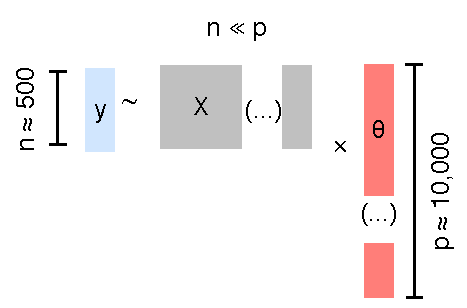
\includegraphics[width=.9\linewidth]{Vis/intractability1} \end{center}


}

\normalsize
\end{column}

\begin{column}{.45\textwidth}
\begin{block}{Col-linearity}
\protect\hypertarget{col-linearity}{}
Variables are somewhat similar to each other
\end{block}

\scriptsize

\onslide<2>{


\begin{center}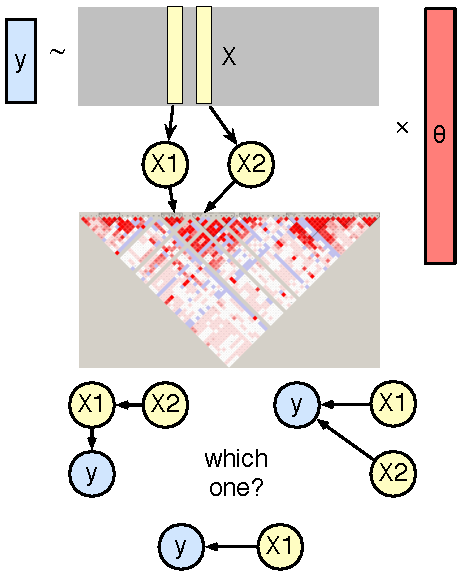
\includegraphics[width=.7\linewidth]{Vis/intractability2} \end{center}


}

\normalsize
\end{column}
\end{columns}

\scriptsize

\normalsize

\scriptsize

\normalsize

\scriptsize

\normalsize
\end{frame}

\begin{frame}[fragile]{A working example - data}
\protect\hypertarget{a-working-example---data}{}
\begin{columns}[T]
\begin{column}{.45\textwidth}
\scriptsize

\begin{center}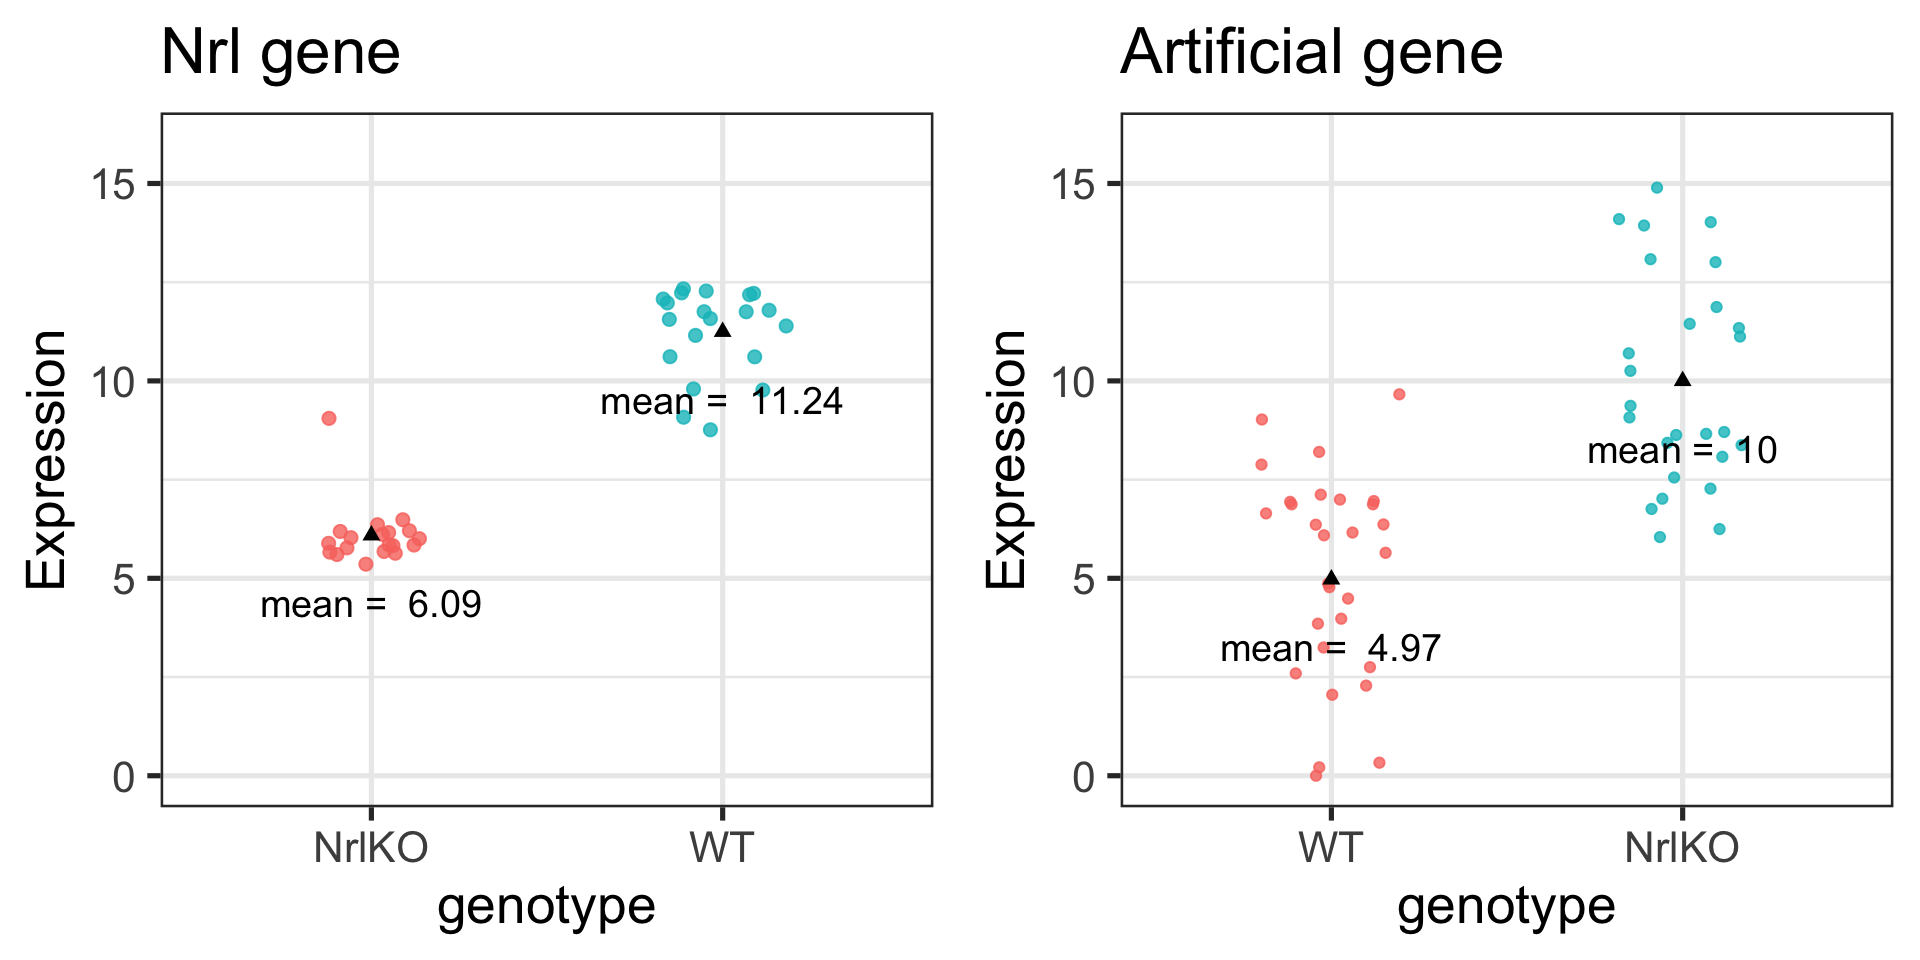
\includegraphics{Fig/supervised/unnamed-chunk-9-1} \end{center}

\normalsize

\scriptsize

\begin{Shaded}
\begin{Highlighting}[]
\FunctionTok{dim}\NormalTok{(y)}
\end{Highlighting}
\end{Shaded}

{[}1{]} 1000 1

\normalsize
\end{column}

\begin{column}{.45\textwidth}
\scriptsize

\begin{center}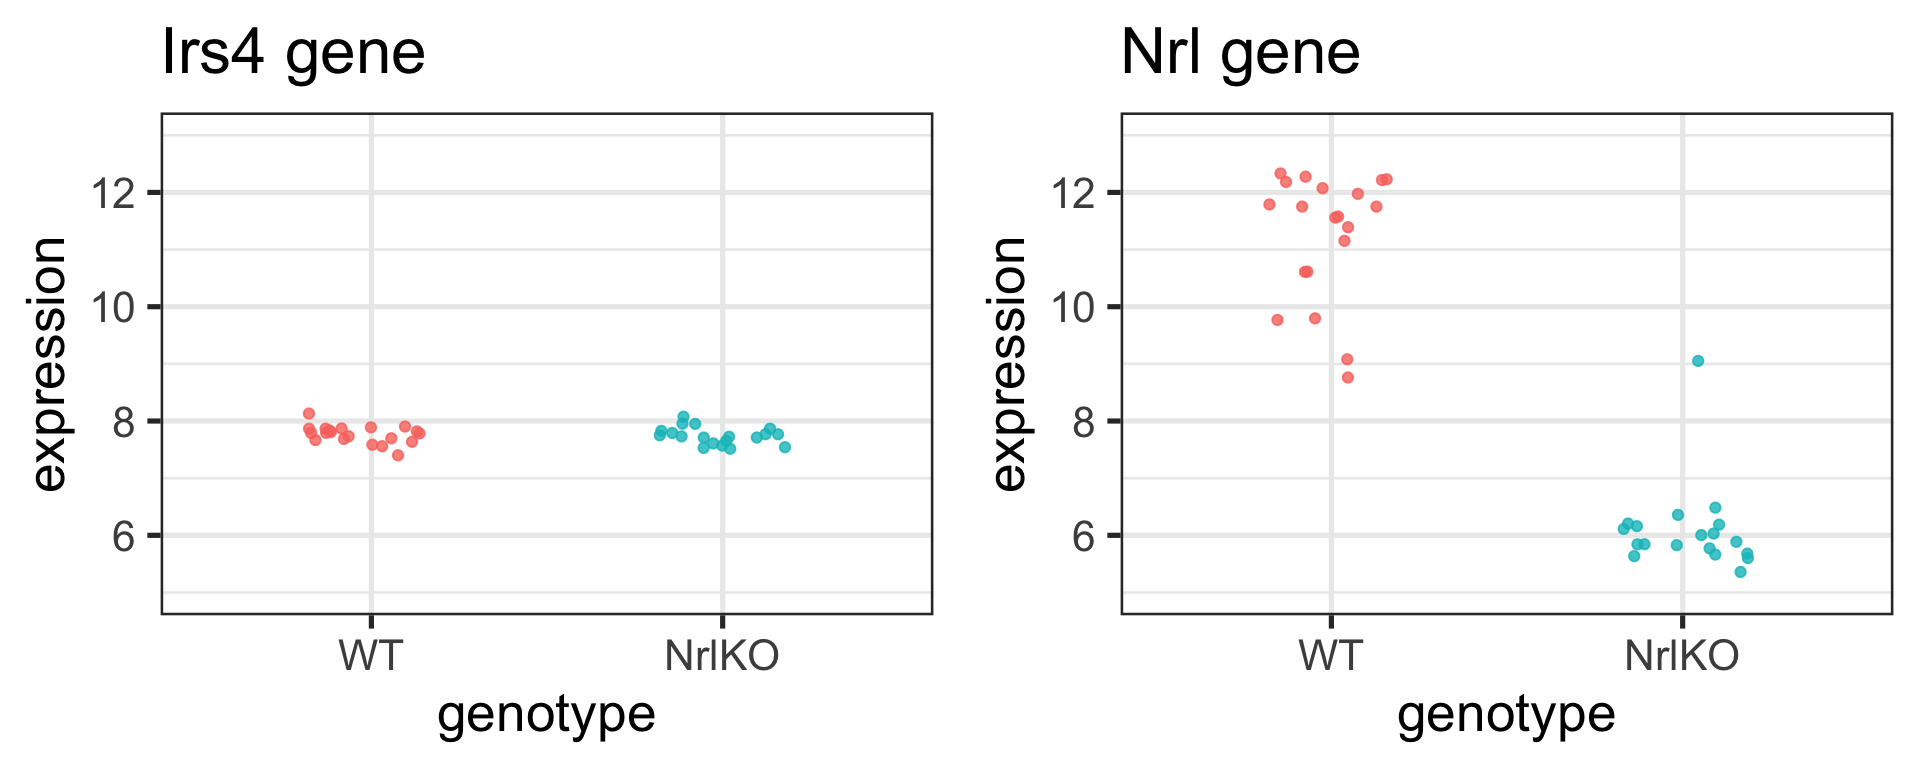
\includegraphics{Fig/supervised/unnamed-chunk-11-1} \end{center}

\normalsize

\scriptsize

\begin{Shaded}
\begin{Highlighting}[]
\FunctionTok{dim}\NormalTok{(X)}
\end{Highlighting}
\end{Shaded}

{[}1{]} 1000 2000

\normalsize
\end{column}
\end{columns}

There are 20 true non-zero variables.
\end{frame}

\begin{frame}[fragile]{True causal variables explain a large fraction of
variation}
\protect\hypertarget{true-causal-variables-explain-a-large-fraction-of-variation}{}
\scriptsize

\begin{Shaded}
\begin{Highlighting}[]
\NormalTok{.lm }\OtherTok{\textless{}{-}} \FunctionTok{lm}\NormalTok{(y }\SpecialCharTok{\textasciitilde{}}\NormalTok{ X[, sim}\SpecialCharTok{$}\NormalTok{causal, }\AttributeTok{drop =} \ConstantTok{FALSE}\NormalTok{] }\SpecialCharTok{{-}} \DecValTok{1}\NormalTok{)}
\end{Highlighting}
\end{Shaded}

\normalsize

\scriptsize

\begin{center}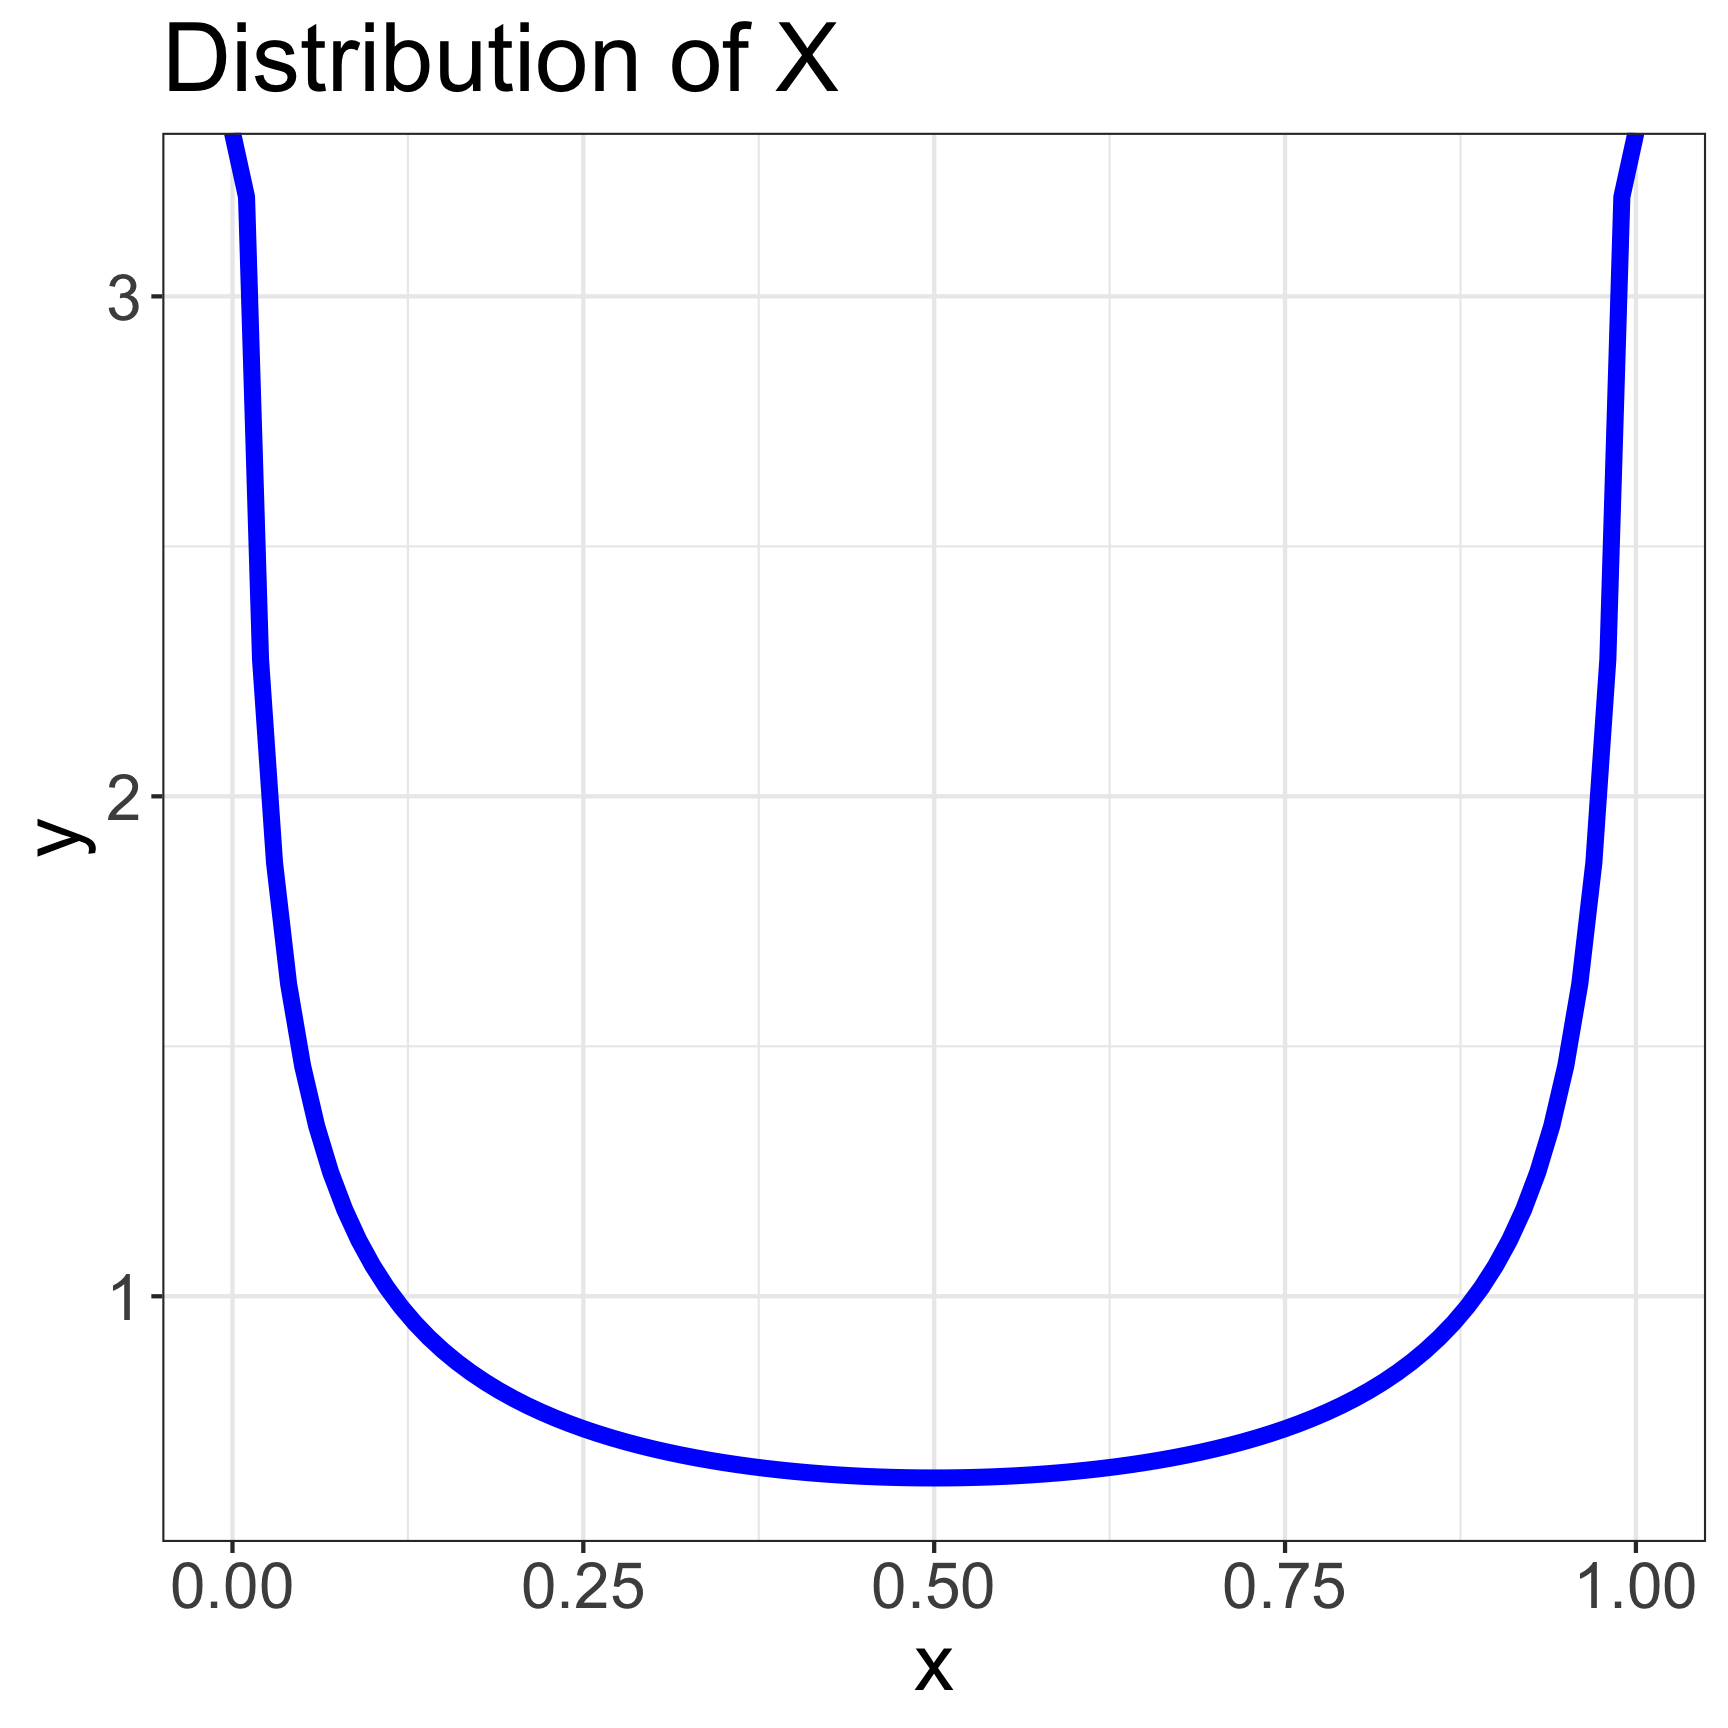
\includegraphics{Fig/supervised/unnamed-chunk-14-1} \end{center}

\normalsize
\end{frame}

\begin{frame}{Variant-by-variant correlations}
\protect\hypertarget{variant-by-variant-correlations}{}
\scriptsize

\begin{center}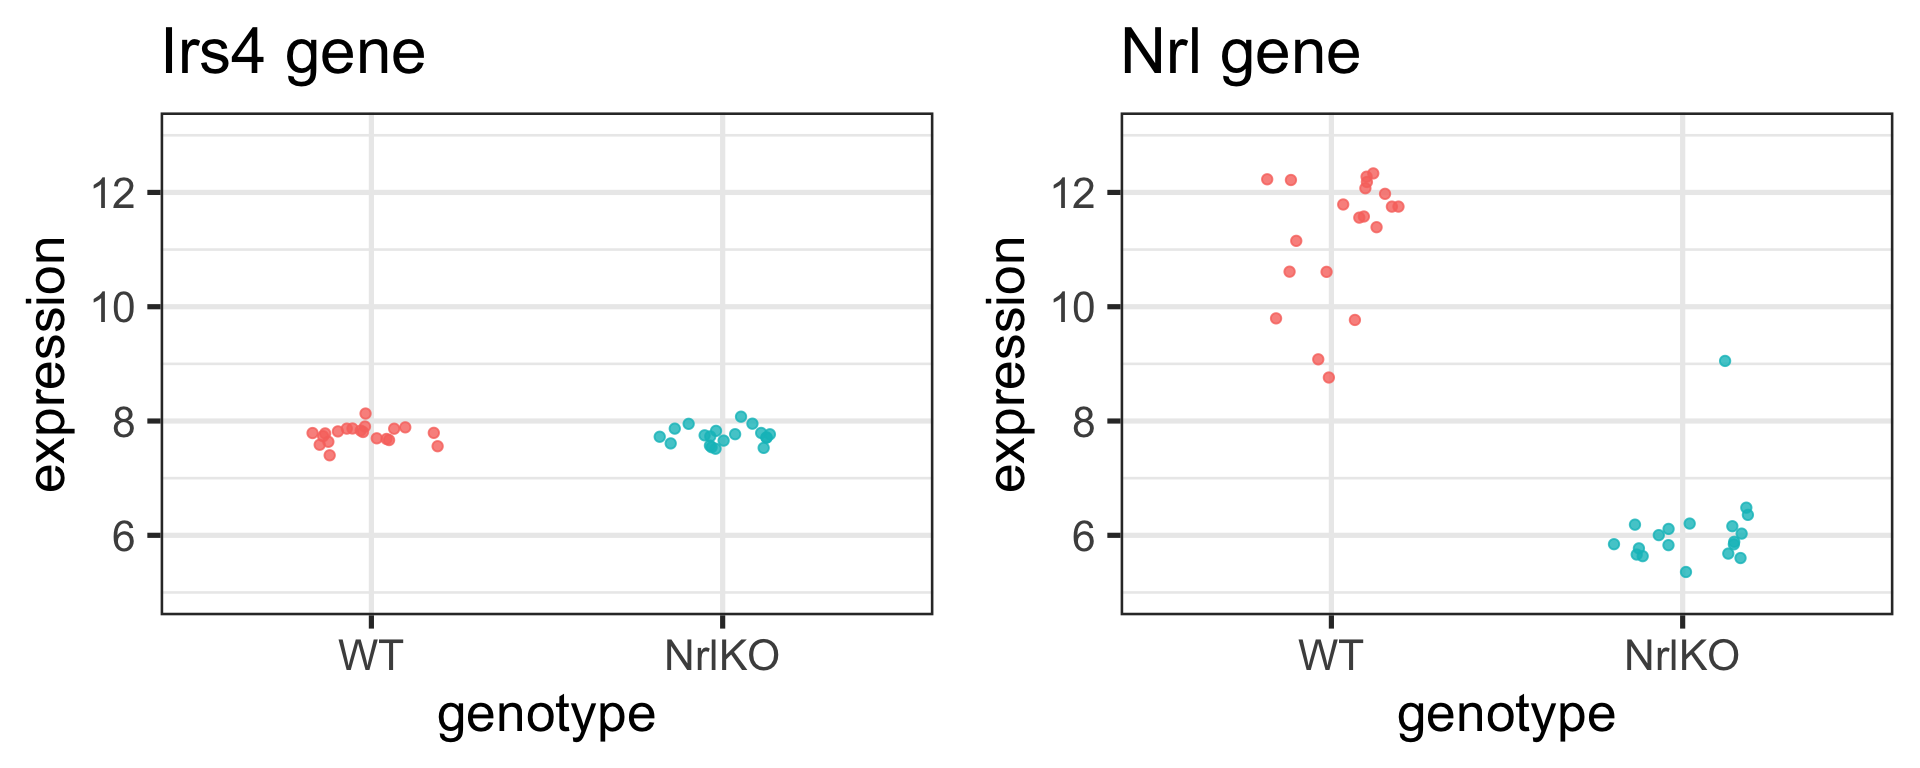
\includegraphics{Fig/supervised/unnamed-chunk-15-1} \end{center}

\normalsize
\end{frame}

\begin{frame}[fragile]{How do we know ``causal'' variables from 2,000
variables?}
\protect\hypertarget{how-do-we-know-causal-variables-from-2000-variables}{}
\begin{itemize}
\tightlist
\item
  Let's try out one by one and rank them by univariate
\end{itemize}

\Large

\texttt{cor.test(x,y)}

\normalsize

\scriptsize

\normalsize

\scriptsize

\normalsize

\scriptsize

\only<2>{


\begin{center}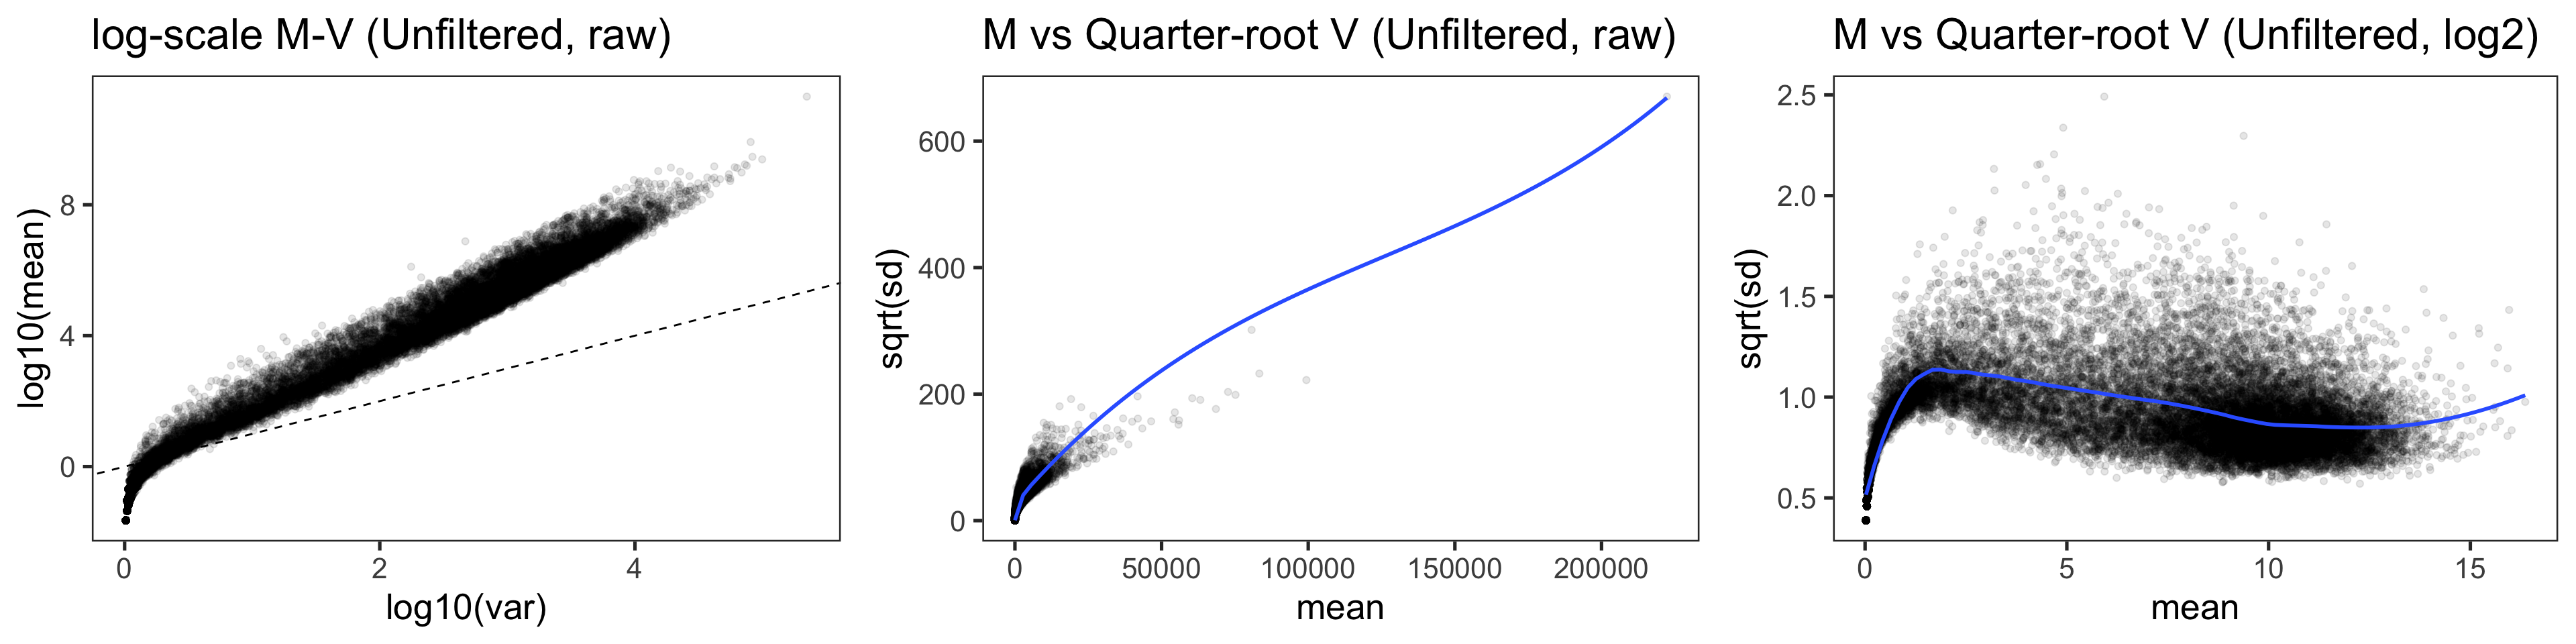
\includegraphics{Fig/supervised/unnamed-chunk-18-1} \end{center}


}

\normalsize

\scriptsize

\only<3>{


\begin{center}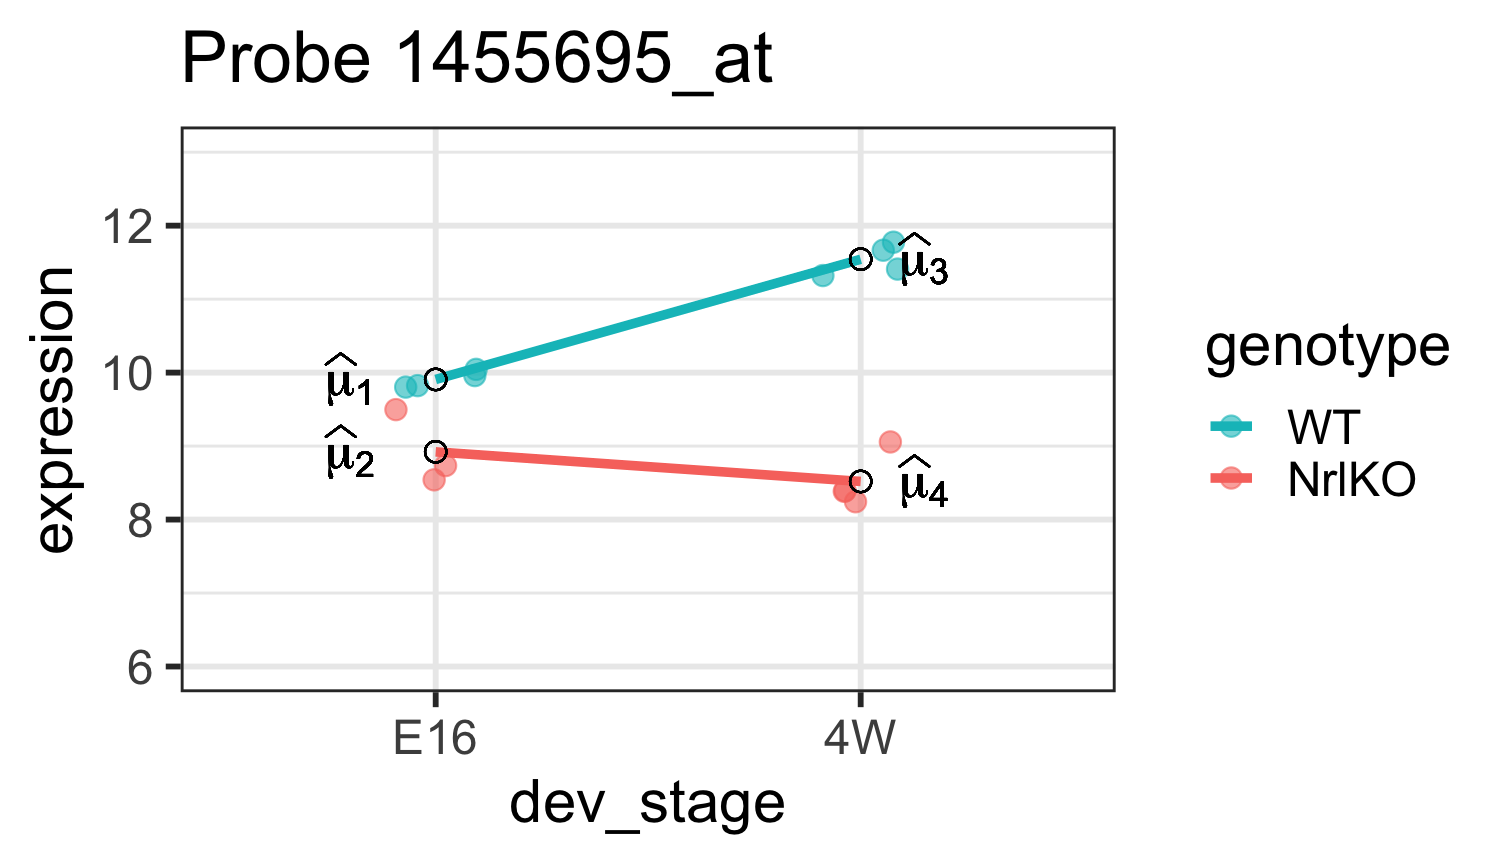
\includegraphics{Fig/supervised/unnamed-chunk-19-1} \end{center}


}

\normalsize

\scriptsize

\only<4>{


\begin{center}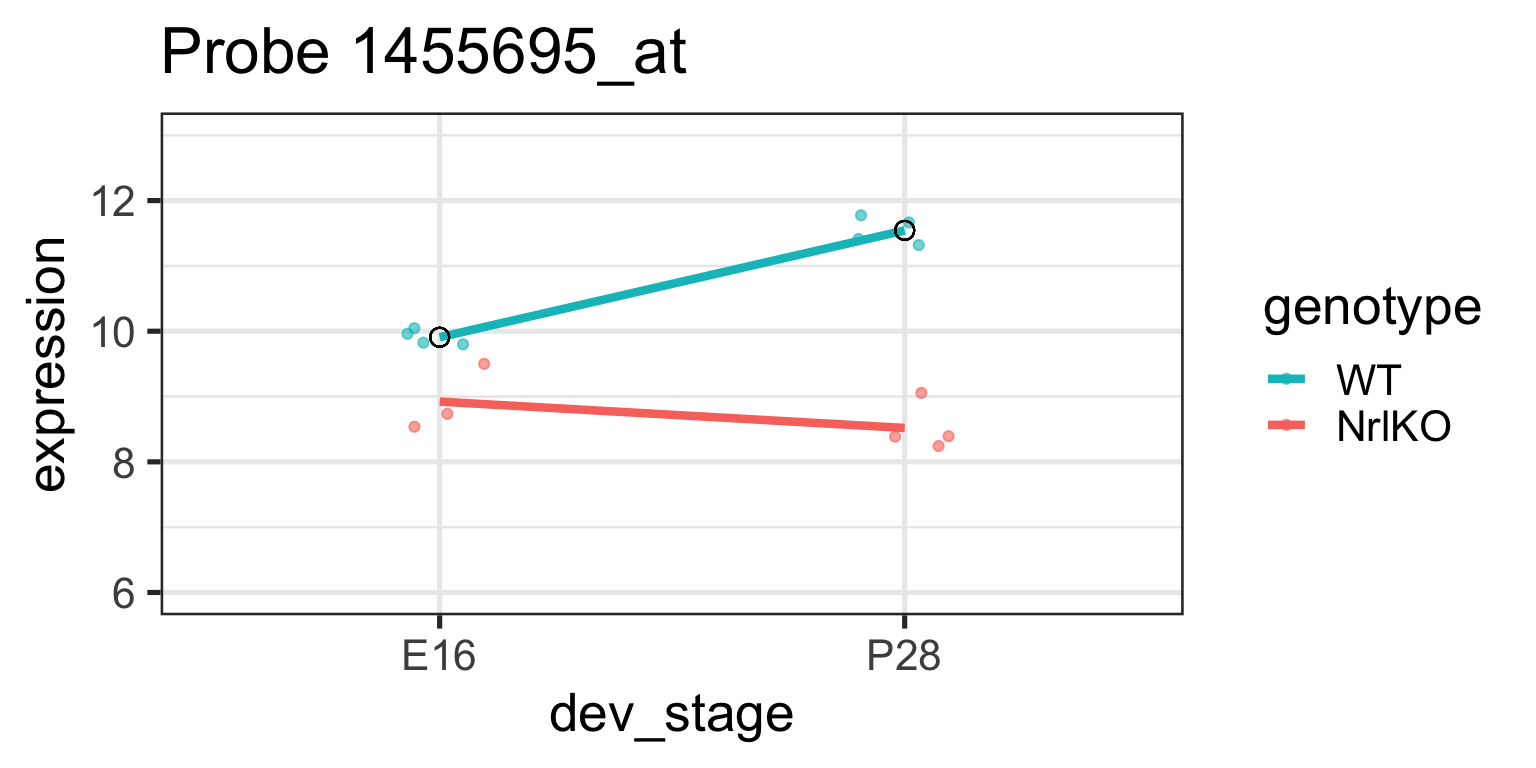
\includegraphics{Fig/supervised/unnamed-chunk-20-1} \end{center}


}

\normalsize

\scriptsize

\only<5>{


\begin{center}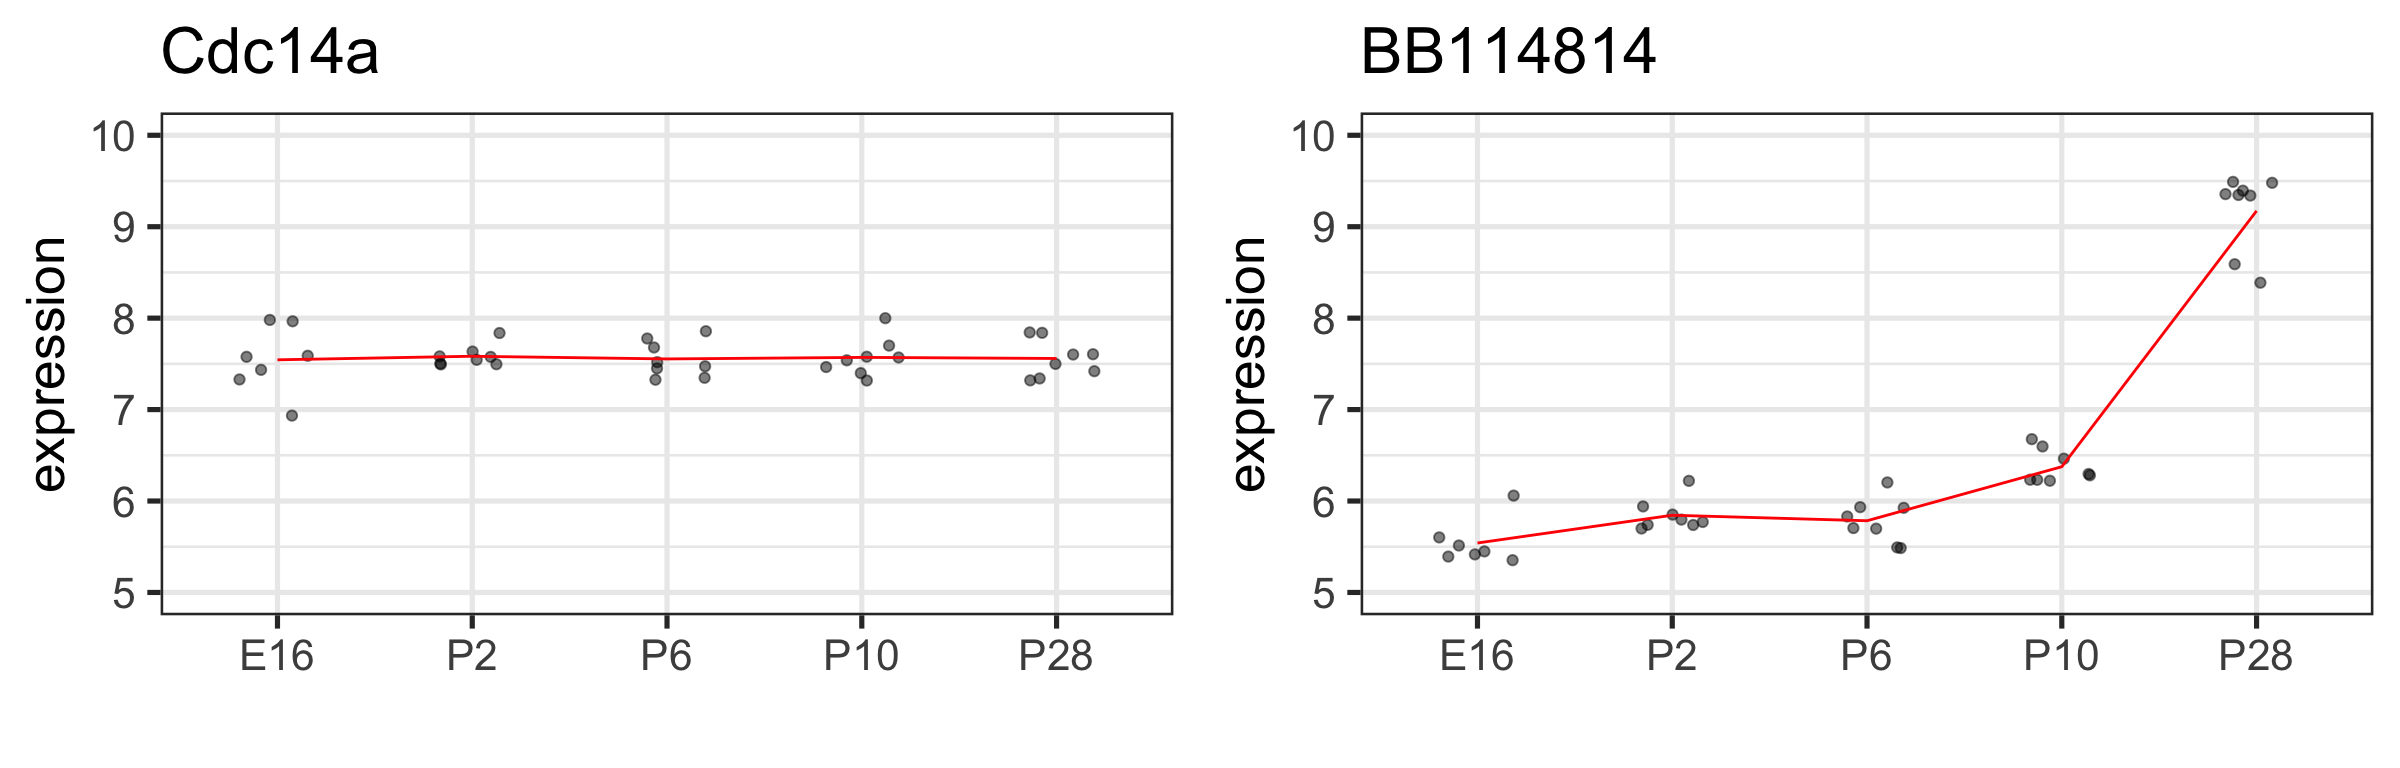
\includegraphics{Fig/supervised/unnamed-chunk-21-1} \end{center}


}

\normalsize

\scriptsize

\only<6>{


\begin{center}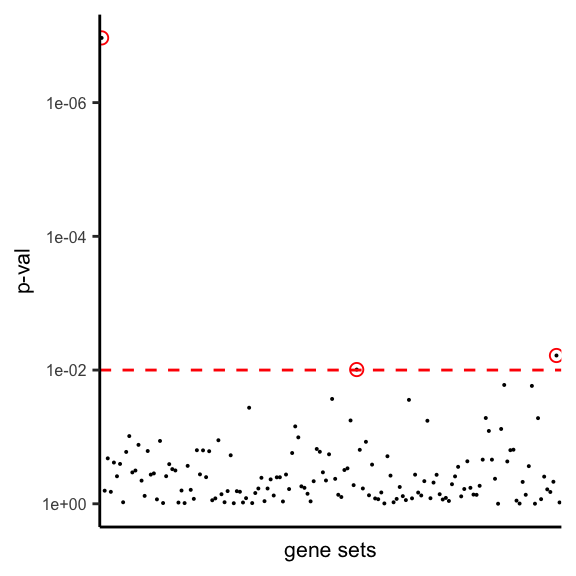
\includegraphics{Fig/supervised/unnamed-chunk-22-1} \end{center}


}

\normalsize
\end{frame}

\begin{frame}{}
\protect\hypertarget{section}{}
\large

\begin{itemize}
\item
  Classical variable selection by univariate (one-by-one) tests will not
  work for a \(p \gg n\) regression problem
\item
  Especially if we have col-linearity in the design matrix \(X\)
\end{itemize}
\end{frame}

\begin{frame}[fragile]{Can we get helped by multivariate regression?}
\protect\hypertarget{can-we-get-helped-by-multivariate-regression}{}
\large

\begin{Shaded}
\begin{Highlighting}[]
\NormalTok{lm.out }\OtherTok{\textless{}{-}} \FunctionTok{lm}\NormalTok{(y }\SpecialCharTok{\textasciitilde{}}\NormalTok{ X }\SpecialCharTok{{-}} \DecValTok{1}\NormalTok{)}
\end{Highlighting}
\end{Shaded}

\normalsize

If you look at the coefficients:

\scriptsize

\begin{longtable}[]{@{}lrrrr@{}}
\toprule
& Estimate & Std. Error & t value &
Pr(\textgreater\textbar t\textbar) \\
\midrule
\endhead
X1 & 1.582654 & 0 & 117826708638 & 0 \\
X2 & -15.949781 & 0 & -134571520044 & 0 \\
X3 & 1.401209 & 0 & 117831497502 & 0 \\
X4 & -5.515155 & 0 & -61749749454 & 0 \\
X5 & 6.827798 & 0 & 66652250040 & 0 \\
X6 & -15.180671 & 0 & -107848045369 & 0 \\
\bottomrule
\end{longtable}

\normalsize

Anything strange?
\end{frame}

\begin{frame}{OLS overfits to the data}
\protect\hypertarget{ols-overfits-to-the-data}{}
\scriptsize

\begin{center}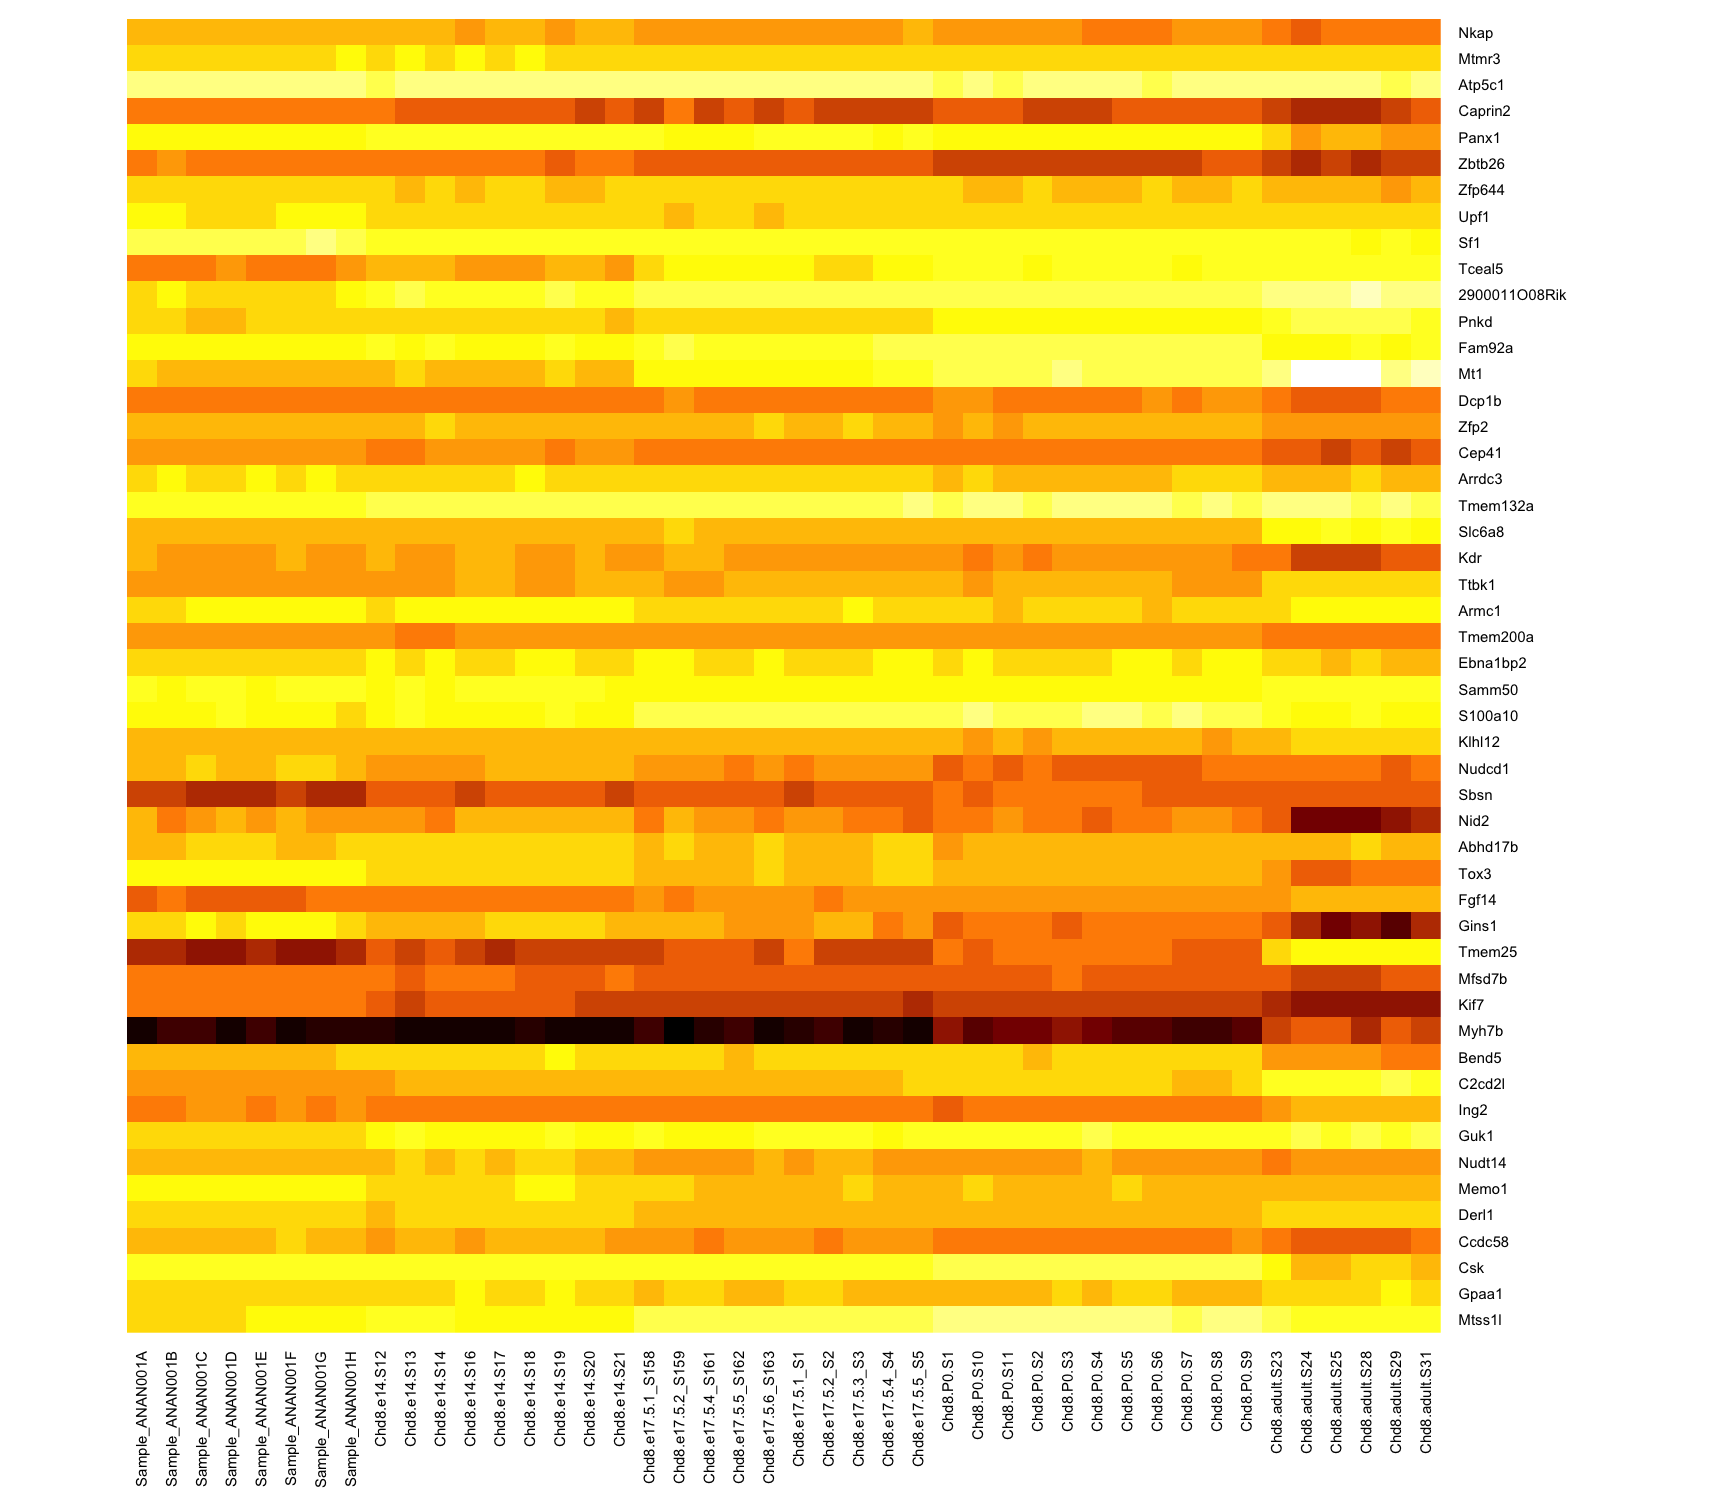
\includegraphics{Fig/supervised/unnamed-chunk-25-1} \end{center}

\normalsize
\end{frame}

\begin{frame}{Can we get helped by multivariate regression?}
\protect\hypertarget{can-we-get-helped-by-multivariate-regression-1}{}
\scriptsize

\begin{center}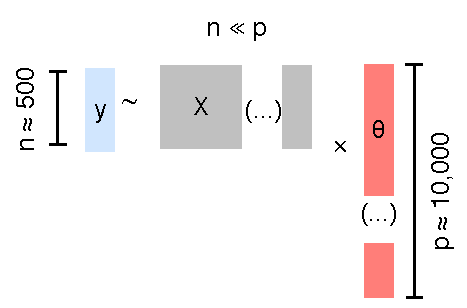
\includegraphics[width=.7\linewidth]{Vis/intractability1} \end{center}

\normalsize

OLS (a.k.a. MLE/MSE) is degenerate if \(p \gg n\)
\end{frame}

\begin{frame}{Variable selection in high-dimensional genotype matrix
(\(n \ll p\))}
\protect\hypertarget{variable-selection-in-high-dimensional-genotype-matrix-n-ll-p}{}
Regression analysis = projecting the observed \(\mathbf{y}\) vector on
to column space of \(\{\mathbf{x}_{j}: j \in[p]\}\), \[
\left(\begin{array}{l}
y_{1}\\
y_{2}\\
\vdots\\
y_{n}
\end{array}\right)
=
\theta_{1} \left(\begin{array}{l}
X_{11}\\
X_{21}\\
\vdots\\
X_{n1}
\end{array}\right) +
\cdots
\theta_{p} \left(\begin{array}{l}
X_{1p}\\
X_{2p}\\
\vdots\\
X_{np}
\end{array}\right).
\] Variable selection = column selection.

\vfill

\begin{itemize}
\item <1-> Intuitive idea : choose the best combination of variables. $\to 2^{p}$ choices (even harder).
\item <2-> Alternative idea : make as many $\theta_{j}$'s nearly zero values.
\item <3-> What prior does: penalize $|\theta_{j}| > 0$ so that only the strong
  enough variables take non-zero values.
\end{itemize}
\end{frame}

\begin{frame}{Bayesian/regularization idea to add the missing
probability component}
\protect\hypertarget{bayesianregularization-idea-to-add-the-missing-probability-component}{}
\large

We've been discussing the conditional likelihood

\[p(\mathbf{y}|X,\boldsymbol{\theta})\]

without a prior probability of regression coefficients,

\[{\color{blue} p(\boldsymbol{\theta})}\]

\textbf{What will be a suitable prior distribution of
\(\boldsymbol{\theta}\)?}
\end{frame}

\begin{frame}{Recall: Reconciling two related concepts -- MLE and MSE}
\protect\hypertarget{recall-reconciling-two-related-concepts-mle-and-mse}{}
Equivalence of maximum-likelihood estimation and mean square error
minimization (isotropic Gaussian error distribution).

\vfill

\textbf{{[}MLE{]}} Find \({\boldsymbol{\theta}}\) maximizing \[
\ln p(\mathbf{y}|X,\boldsymbol{\theta})
= - \frac{1}{2\sigma^{2}} \sum_{i=1}^{n} (y_{i} - \mathbf{x}_{i} \boldsymbol{\theta})^{2} + \textrm{const.}
\] \emph{without prior contribution of parameter, and \(\sigma\) is
known.}

\vfill

\textbf{{[}MSE{]}} Find \(\boldsymbol{\theta}\) minimizing \[
\sum_{i=1}^{n} (y_{i} - \mathbf{x}_{i} \boldsymbol{\theta})^{2}.
\]
\end{frame}

\begin{frame}{Ridge regression, a linear regression with Gaussian prior
(L2)}
\protect\hypertarget{ridge-regression-a-linear-regression-with-gaussian-prior-l2}{}
Prior distribution \[
p(\boldsymbol{\theta}) = \mathcal{N}\!\left(\boldsymbol{\theta}|\mathbf{0}, \lambda^{-1} I\right) \propto \exp\left(-\frac{\lambda}{2}\|\boldsymbol{\theta}\|^{2}\right)
\] where \large
\[\|\boldsymbol{\theta}\|^{2} = \sum_{j=1}^{p} \theta_{j}^{2},\,\textsf{\color{blue}L2-norm}.\]

\normalsize

Maximize \[
\ln p(\mathbf{y}|X,\boldsymbol{\theta}) + \ln p(\boldsymbol{\theta}|\lambda)
= - \frac{1}{2\sigma^{2}} \sum_{i=1}^{n} (y_{i} - \mathbf{x}_{i} \boldsymbol{\theta})^{2}
- \frac{\lambda}{2} \|\boldsymbol{\theta}\|^{2}
\]

Minimize \(L_{2}\)-regularized error \[
\sum_{i=1}^{n} (y_{i} - \mathbf{x}_{i} \boldsymbol{\theta})^{2}
+ \frac{\lambda}{2} \|\boldsymbol{\theta}\|^{2}
\]
\end{frame}

\begin{frame}{Lasso regression, a linear regression with Laplace prior
(L1)}
\protect\hypertarget{lasso-regression-a-linear-regression-with-laplace-prior-l1}{}
Prior distribution \[
p(\boldsymbol{\theta}) = \textsf{Laplace}(\boldsymbol{\theta}| \lambda) \propto \exp\left(-\lambda\|\boldsymbol{\theta}\|_{1}\right)
\] where \large
\[\|\boldsymbol{\theta}\|_{1} = \sum_{j=1}^{p} |\theta_{j}|,\,\textsf{\color{blue}L1-norm}.\]

\normalsize

Maximize \[
\ln p(\mathbf{y}|X,\boldsymbol{\theta}) + \ln p(\boldsymbol{\theta}|\lambda)
= - \frac{1}{2\sigma^{2}} \sum_{i=1}^{n} (y_{i} - \mathbf{x}_{i} \boldsymbol{\theta})^{2}
- \lambda \|\boldsymbol{\theta}\|_{1}
\]

Minimize \(L_{1}\)-regularized error \[
\sum_{i=1}^{n} (y_{i} - \mathbf{x}_{i} \boldsymbol{\theta})^{2}
+ \lambda \|\boldsymbol{\theta}\|_{1}
\]

(Tibshirani, 1996)
\end{frame}

\begin{frame}{Geometric intuition of regularization.}
\protect\hypertarget{geometric-intuition-of-regularization.}{}
Consider a simple regression model:
\(y_{i} = \theta_{1} X_{i1} + \theta_{2} X_{i2}\).

\vfill

\only<1-2>{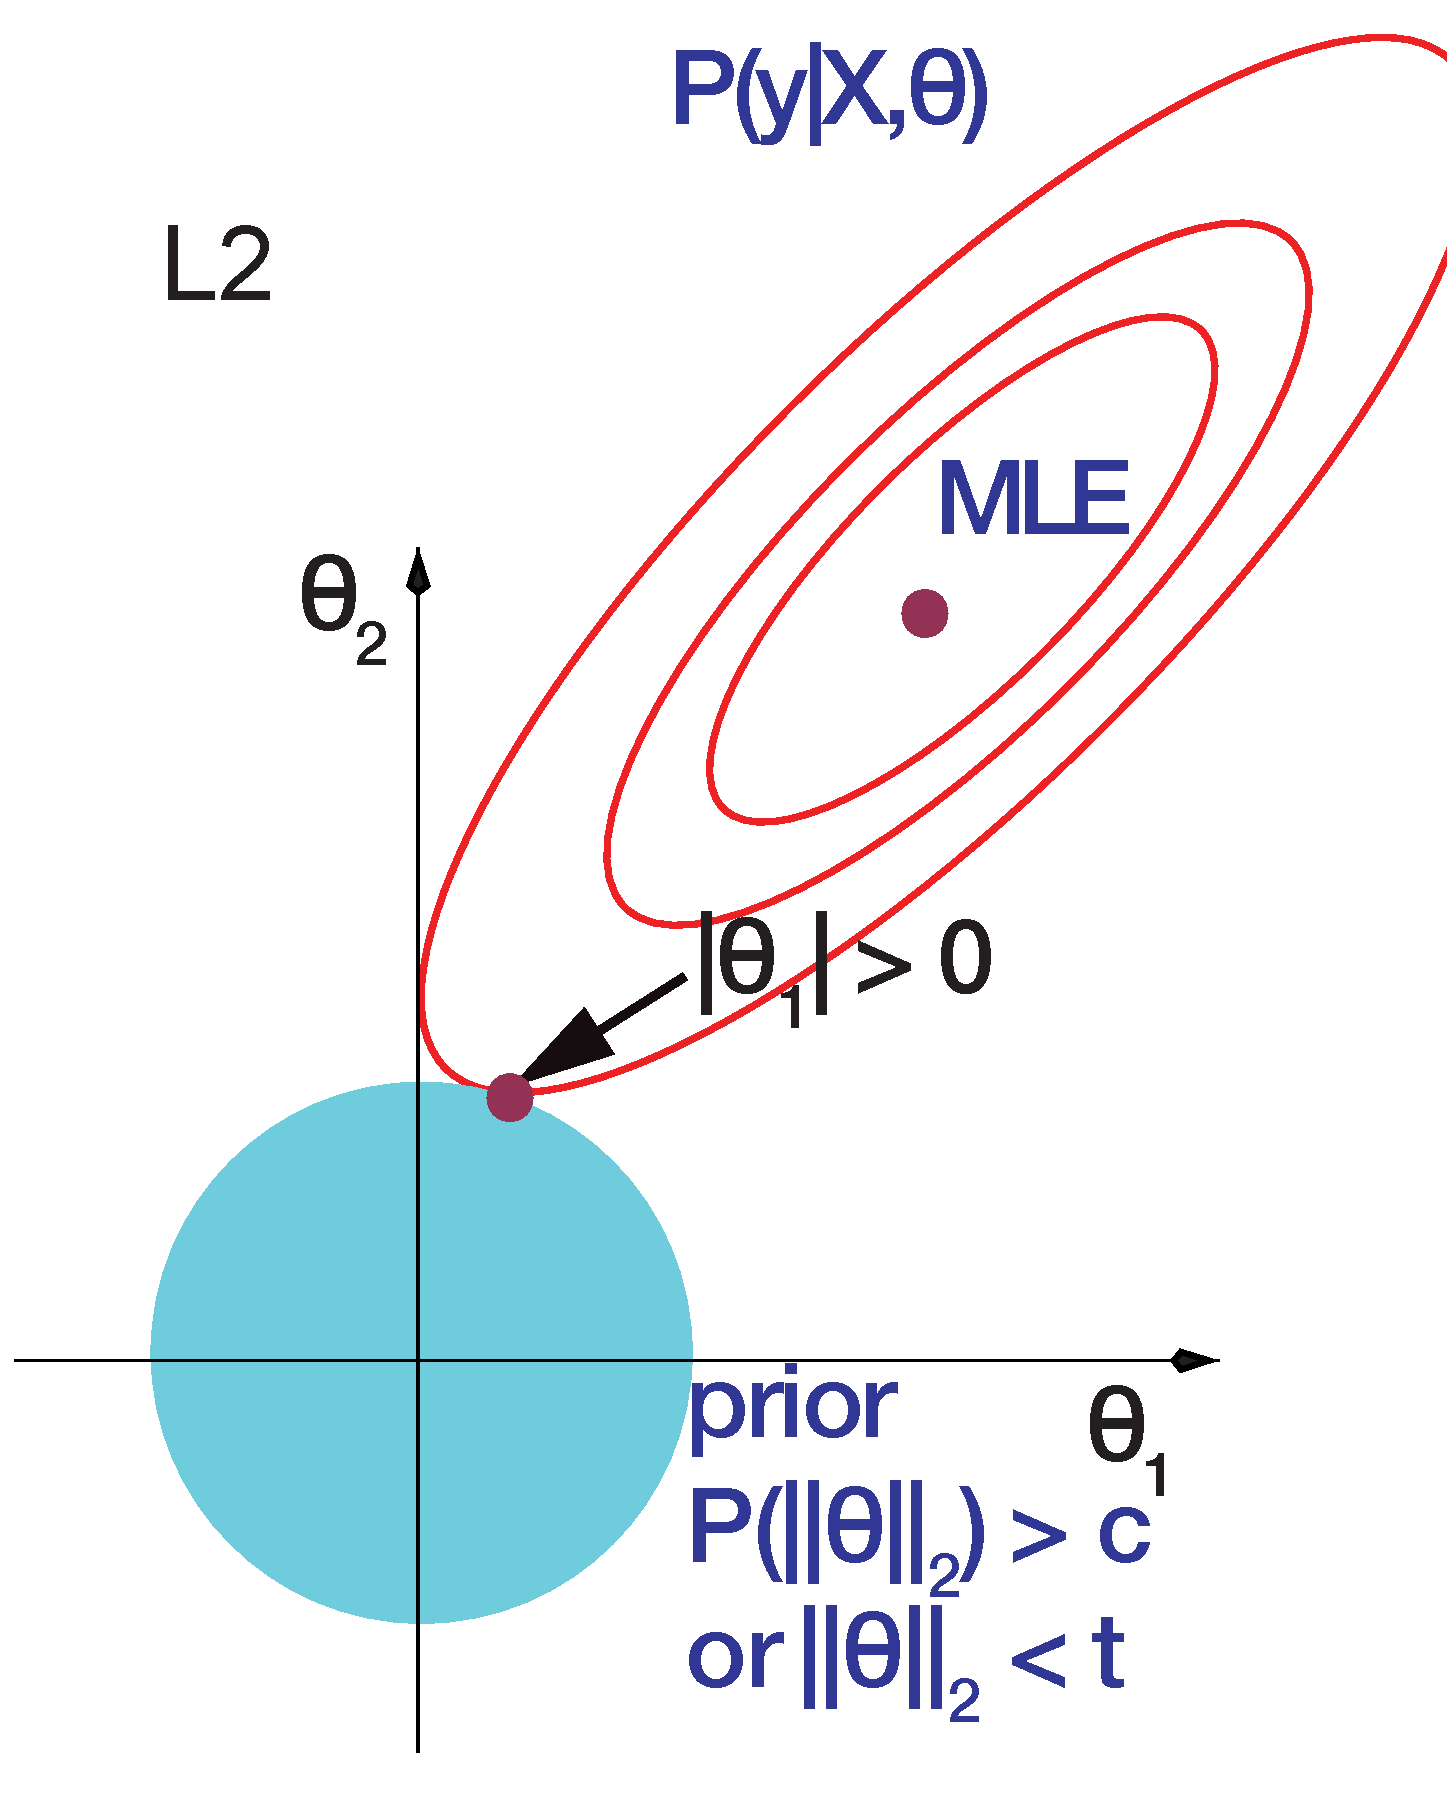
\includegraphics[width=.35\textwidth]{Vis/Geom_L2.pdf}}
\only<2>{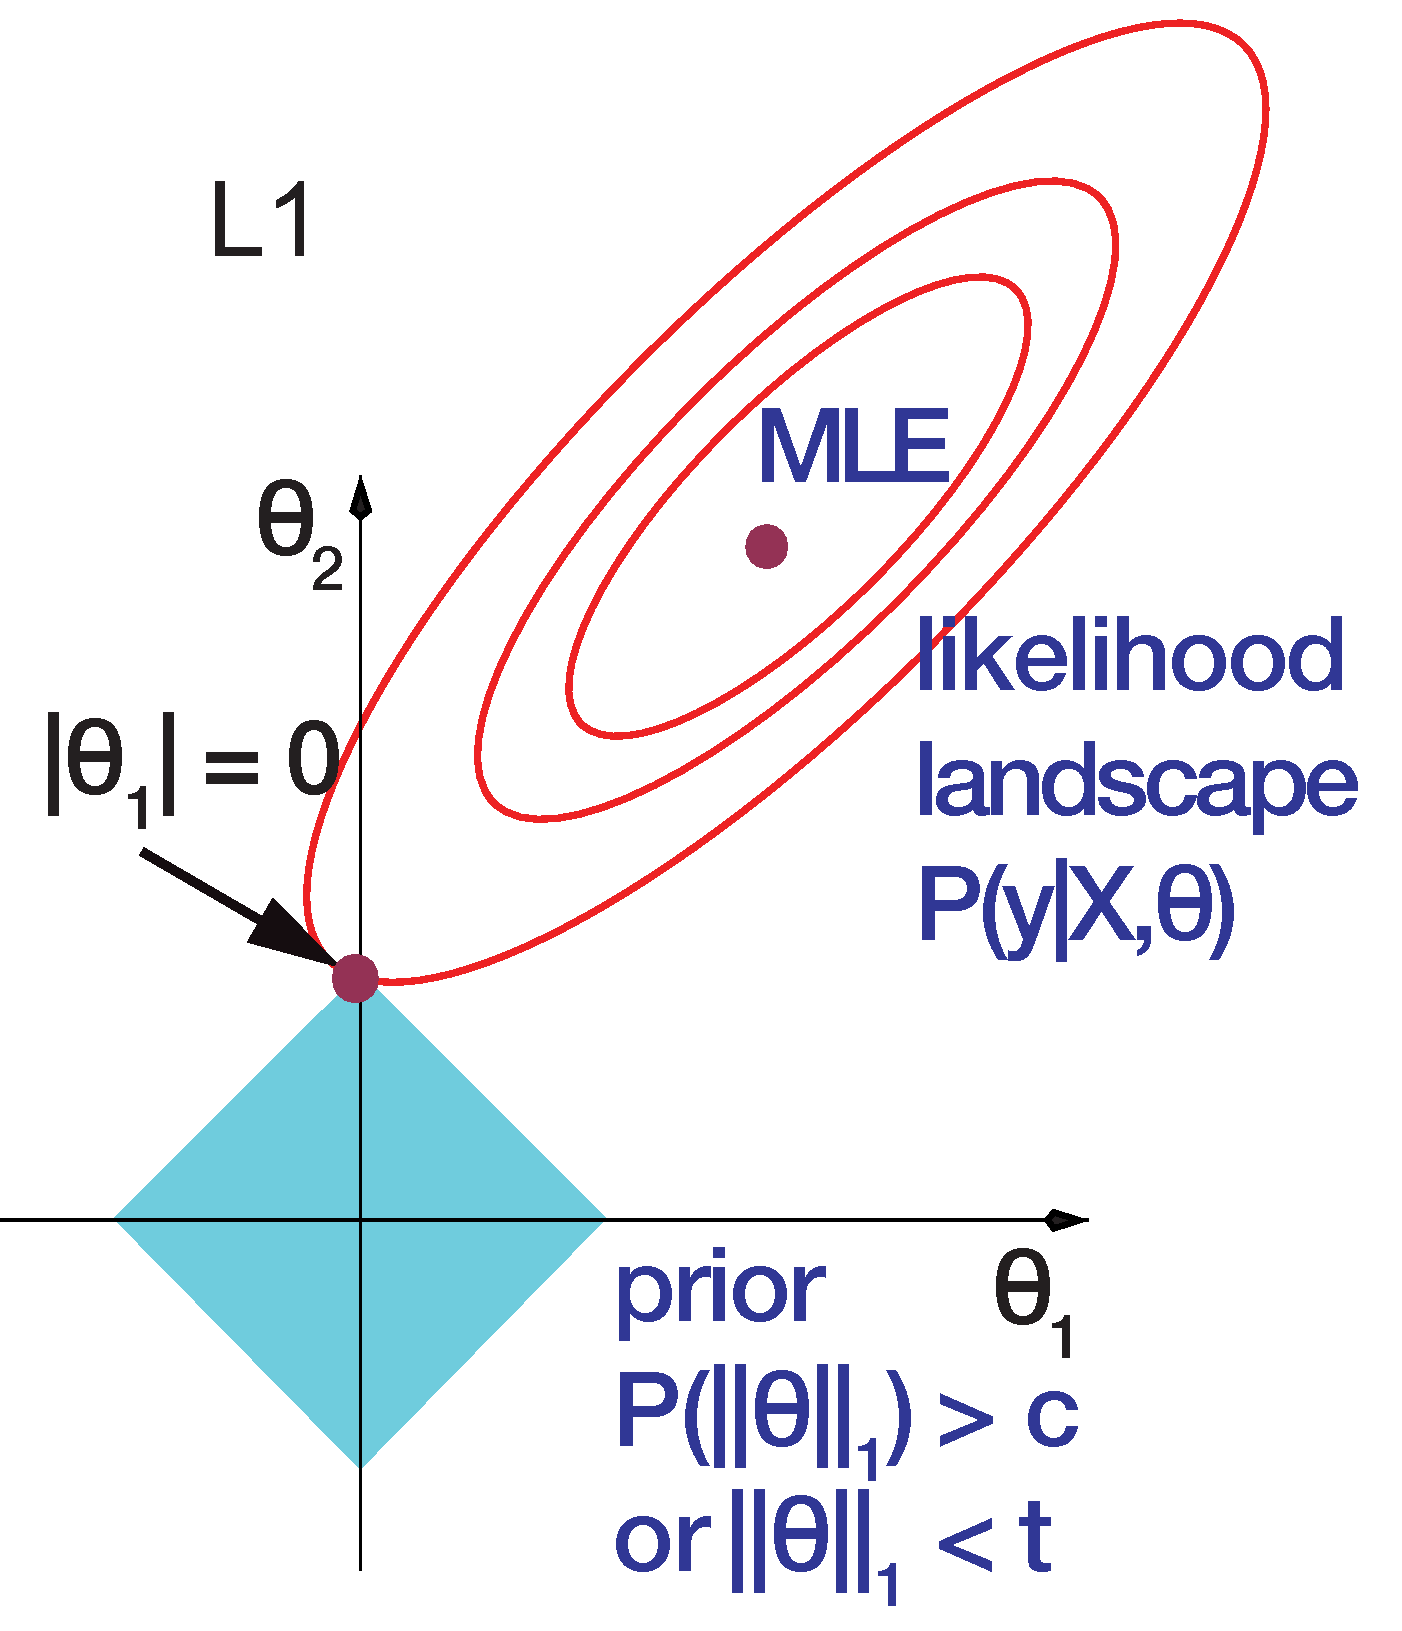
\includegraphics[width=.35\textwidth]{Vis/Geom_L1.pdf}}
\only<3>{\centerline{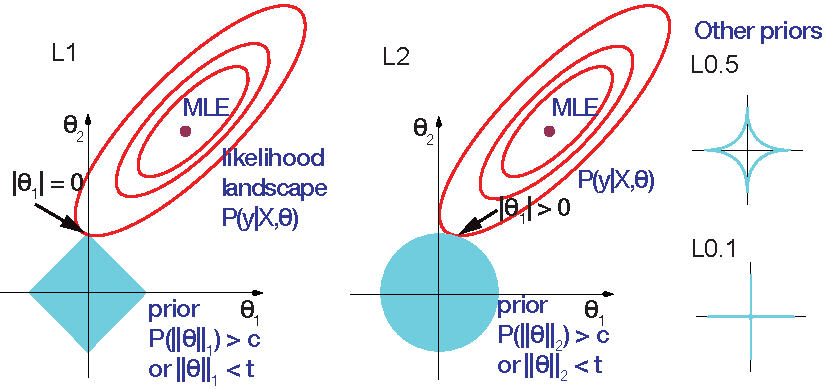
\includegraphics[width=.75\textwidth]{Vis/L1L2.pdf}}}

\vfill

\only<3>{
\begin{itemize}
\item Both regularization priors shrink the coefficients toward zero.
\item But only L1 can effectively "select" variables; although we want $L_{0}$.
\end{itemize}

\flushleft{\tiny Hastie, Tibshirani, Friedman, {\it The Elements of Statistical Learning.}}
}
\end{frame}

\begin{frame}{Posterior inference of the regularized regression models}
\protect\hypertarget{posterior-inference-of-the-regularized-regression-models}{}
Our goal is to estimate (1) posterior distribution \[
p(\boldsymbol{\theta}|\mathbf{y}, X) = \frac{p(\mathbf{y}|X,\boldsymbol{\theta})p(\boldsymbol{\theta})}{p(\boldsymbol{y}|X)}.
\]

Then (2) using \(p(\boldsymbol{\theta}|\mathbf{y},X)\), predict
\(p(\mathbf{y}^{\star}|\mathbf{y},X)\) by averaging over all possible
\(\boldsymbol{\theta}\) sampled from the estimated posterior
distribution.

\vfill

\begin{itemize}
\item
  Usually posterior prediction (2) is can be easily simulated with
  accurate estimation of posterior distribution (1).
\item
  Posterior inference can be done analytically or not, depending on the
  choice of
  \(p(\boldsymbol{\theta})\)\footnote{We term prior $p(\boldsymbol{\theta})$ a {\it conjugate prior} if its posterior $p(\boldsymbol{\theta}|\mathbf{y},X)$ is of the same type of distribution.}.
\end{itemize}
\end{frame}

\begin{frame}{We can find an analytical solution in L2-regularized
regression}
\protect\hypertarget{we-can-find-an-analytical-solution-in-l2-regularized-regression}{}
\[
\ln p(\mathbf{\boldsymbol{\theta}}|\mathbf{y},X) =
-\frac{1}{2\sigma^{2}} (\mathbf{y} - X\boldsymbol{\theta})^{\top}(\mathbf{y} - X\boldsymbol{\theta}) - \frac{\lambda}{2} \boldsymbol{\theta}^{\top}\boldsymbol{\theta} + \textrm{const.}
\]

\onslide<2->{
By taking derivative with respect to $\boldsymbol{\theta}$ and setting it the zero vector:
$$
\nabla_{\boldsymbol{\theta}} = -\frac{1}{\sigma^{2}} X^{\top}(\mathbf{y} - X\boldsymbol{\theta})
-\lambda \boldsymbol{\theta} = 0
$$
}

\vfill

\onslide<3->{
Rearranging the equation:
$$
X^{\top}\mathbf{y} = (X^{\top}X + \lambda\sigma^{2} I) \boldsymbol{\theta}\,
\implies\,
\hat{\boldsymbol{\theta}} = (X^{\top}X + \lambda\sigma^{2} I)^{-1} X^{\top}\mathbf{y}
$$
}

\onslide<4>{
\textit{Remark}: For $n \ll p$, the inverse $(X^{\top}X)^{-1}$ may not exists, but $(X^{\top}X + \lambda\sigma^{2}I)^{-1}$ can exist with a proper $\lambda$.
}
\end{frame}

\begin{frame}[fragile]{We can solve L1-regularized regression
numerically}
\protect\hypertarget{we-can-solve-l1-regularized-regression-numerically}{}
\begin{columns}[T]
\begin{column}{.45\textwidth}
\scriptsize

\onslide<1->{


\begin{center}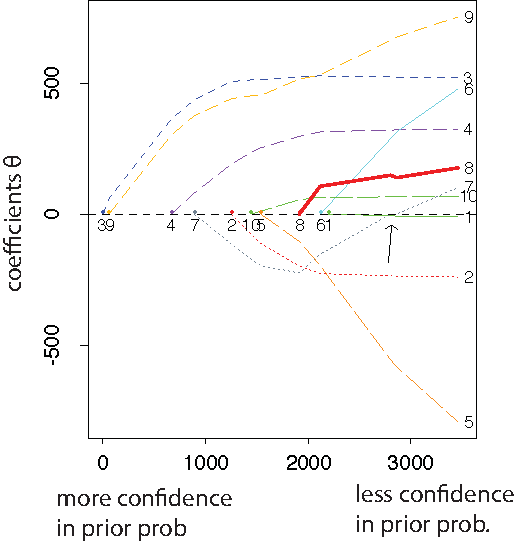
\includegraphics[width=.9\textwidth]{Vis/LARS} \end{center}


}

\normalsize
\end{column}

\begin{column}{.45\textwidth}
Algorithms from statistics:

\begin{itemize}
\item
  Efron \emph{et al.} Least Angle Regression (2002)
\item
  Hans \emph{et al.}, Shotgun search (2007)
\item
  Friedman \emph{et al.}, \texttt{glmnet} (2010)
\end{itemize}

From ML:

\begin{itemize}
\item
  Figueiredo \emph{et al.} PAMI (2003)
\item
  Seeger \emph{et al.} JMLR (2008)
\end{itemize}
\end{column}
\end{columns}
\end{frame}

\begin{frame}{In practice, the greedy algorithm of \texttt{glmnet} works
so well}
\protect\hypertarget{in-practice-the-greedy-algorithm-of-glmnet-works-so-well}{}
Goal:

\[
\min_{\boldsymbol{\theta}} \quad
\overbrace{(\mathbf{y} - X\boldsymbol{\theta})^{\top}(\mathbf{y} - X\boldsymbol{\theta})}^{\textsf{\color{blue} RSS}} + \underbrace{\lambda \alpha \|\boldsymbol{\theta}\|_{1}}_{\textsf{\color{red} variable selection}} + \underbrace{\lambda (1 - \alpha) \|\boldsymbol{\theta}\|_{2}}_{\textsf{\color{magenta} shrinkage}}
\]

\onslide<2->{
The variable-by-variable update equation makes sense:

For each $\theta_{j}$,
}

\only<2>{$$
\hat{\theta}_{j}^{\textsf{glmnet}} \gets
\frac{S\left(
\sum_{i=1}^{n} X_{ij} (y_{i} - \hat{y}_{i}^{(-j)}),
\lambda\alpha
\right)}
{ \sum_{i=1}^{n} X_{ij}^{2} +\lambda (1- \alpha) }
\quad\textsf{vs.}\quad
\theta_{j}^{\textsf{MLE}} \gets
\frac{
\sum_{i=1}^{n} X_{ij} \left(
y_{i} - \sum_{k\neq j} X_{ik}\hat{\theta}_{k}
\right)}
{\sum_{i=1}^{n} X_{ij}^{2}}
$$
\tiny
Friedman {\it et al.}, Regularization Paths for Generalized Linear Models via Coordinate Descent (2010)
}

\only<3>{$$
\hat{\theta}_{j} \gets
\frac{\overset{\textsf{\color{red} threshold}}{S}
\left(
\sum_{i=1}^{n} X_{ij} \overbrace{(y_{i} - y_{i}^{(-j)})}^{\textsf{\color{red} residual w/o the variable } \theta_{j} },
\lambda\alpha
\right)}
{ \sum_{i=1}^{n} X_{ij}^{2} + \underbrace{\lambda (1- \alpha)}_{\textsf{\color{magenta} shrinkage}}}
$$
where $S(z, \tau)$ will set it to zero if $|z| < \tau$.
}
\end{frame}

\begin{frame}{Cross-validation: How do we tune hyper-parameters (e.g.,
\(\lambda\))?}
\protect\hypertarget{cross-validation-how-do-we-tune-hyper-parameters-e.g.-lambda}{}
\begin{enumerate}
\item
  Divide the total training data
  \(\mathcal{D}^{\textsf{train}} = \{(X,y)\}\) into two parts:

  \begin{itemize}
  \item
    \begin{enumerate}
    [(1)]
    \tightlist
    \item
      cross-validation training \(\{(X,y)\}\) and
    \end{enumerate}
  \item
    \begin{enumerate}
    [(1)]
    \setcounter{enumii}{1}
    \tightlist
    \item
      CV testing data \(\{(X^\star,y^\star)\}\)
    \end{enumerate}
  \end{itemize}
\item
  For each different \((\lambda, \alpha)\) combination,

  \begin{itemize}
  \item
    Train coefficients \(\theta\) using CV training
    \(\{(X,y)\} \subset \mathcal{D}^{\textsf{train}}\)
  \item
    Test how well \(\sum_{j} X^{\star}_{ij} \hat{\theta}_{j}\) predicts
    \(y^\star\)?
  \end{itemize}
\item
  Choose the optimal \((\lambda^\star, \alpha^\star)\)
\end{enumerate}
\end{frame}

\begin{frame}[fragile]{How do we tune hyper-parameters (e.g.,
\(\lambda\))?}
\protect\hypertarget{how-do-we-tune-hyper-parameters-e.g.-lambda}{}
Well, in \texttt{R}, we simply run

\begin{columns}[T]
\begin{column}{.35\textwidth}
\large

\begin{Shaded}
\begin{Highlighting}[]
\NormalTok{glm.cv.out }\OtherTok{\textless{}{-}}
\NormalTok{ glmnet}\SpecialCharTok{::}\FunctionTok{cv.glmnet}\NormalTok{(X,}
\NormalTok{          y,}
          \AttributeTok{nfolds=}\DecValTok{5}\NormalTok{,}
          \AttributeTok{alpha=}\DecValTok{1}\NormalTok{)}
\end{Highlighting}
\end{Shaded}

\normalsize
\end{column}

\begin{column}{.55\textwidth}
\scriptsize

\only<3>{


\begin{center}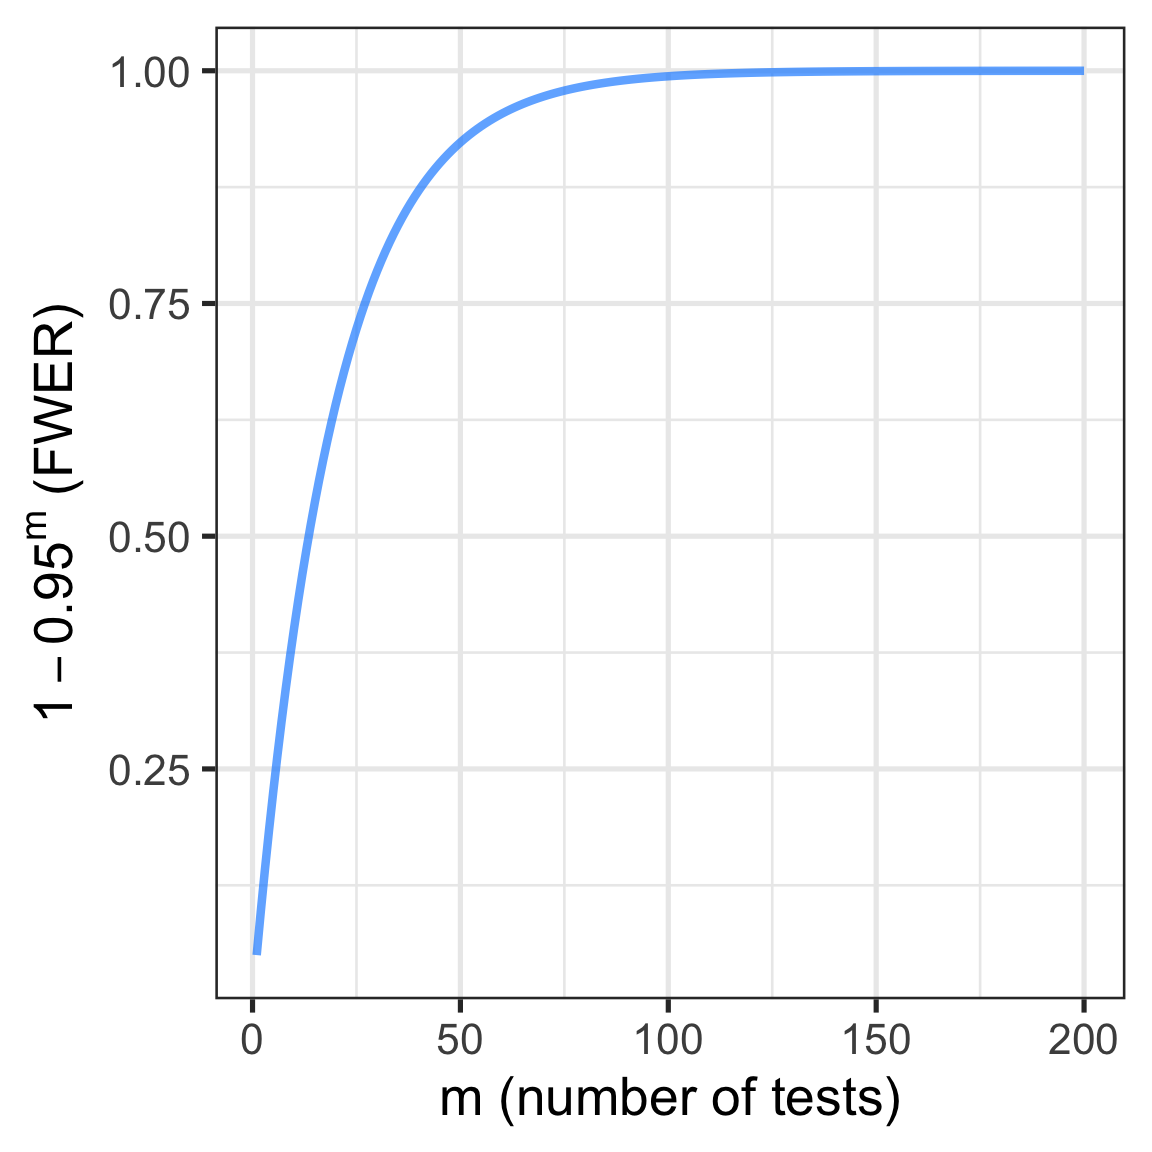
\includegraphics{Fig/supervised/unnamed-chunk-29-1} \end{center}


}

\normalsize
\end{column}
\end{columns}
\end{frame}

\begin{frame}{Revisit our working example with L1-regularization
(\texttt{glmnet})}
\protect\hypertarget{revisit-our-working-example-with-l1-regularization-glmnet}{}
\scriptsize

\begin{center}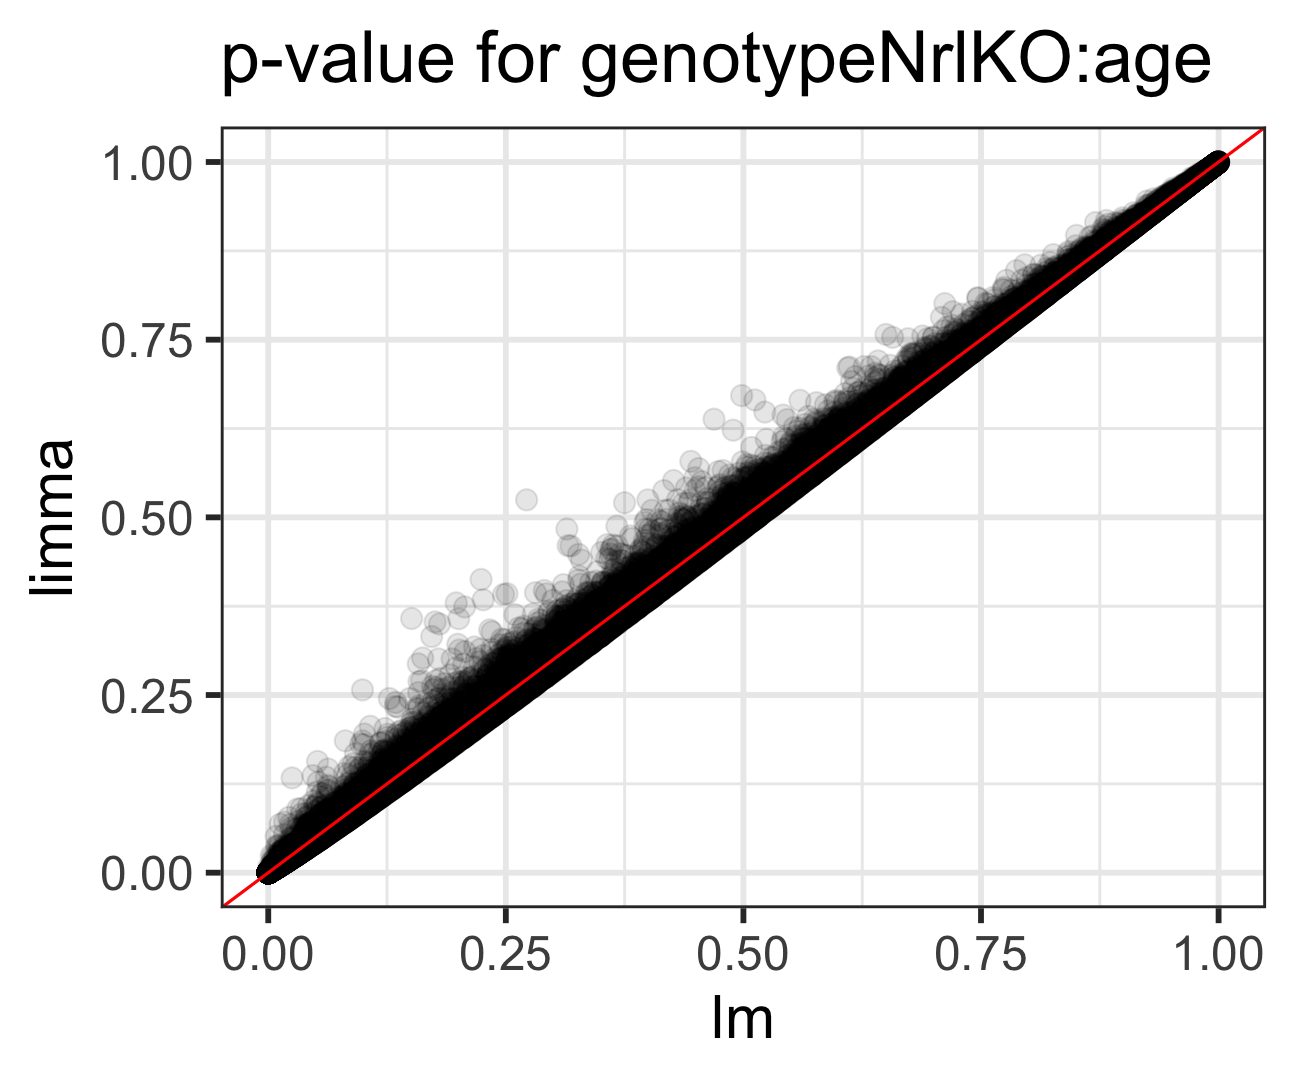
\includegraphics{Fig/supervised/unnamed-chunk-30-1} \end{center}

\normalsize
\end{frame}

\begin{frame}{At the optimal \(\lambda\) found by \texttt{cv.glmnet}}
\protect\hypertarget{at-the-optimal-lambda-found-by-cv.glmnet}{}
\scriptsize

\normalsize

\scriptsize

\begin{center}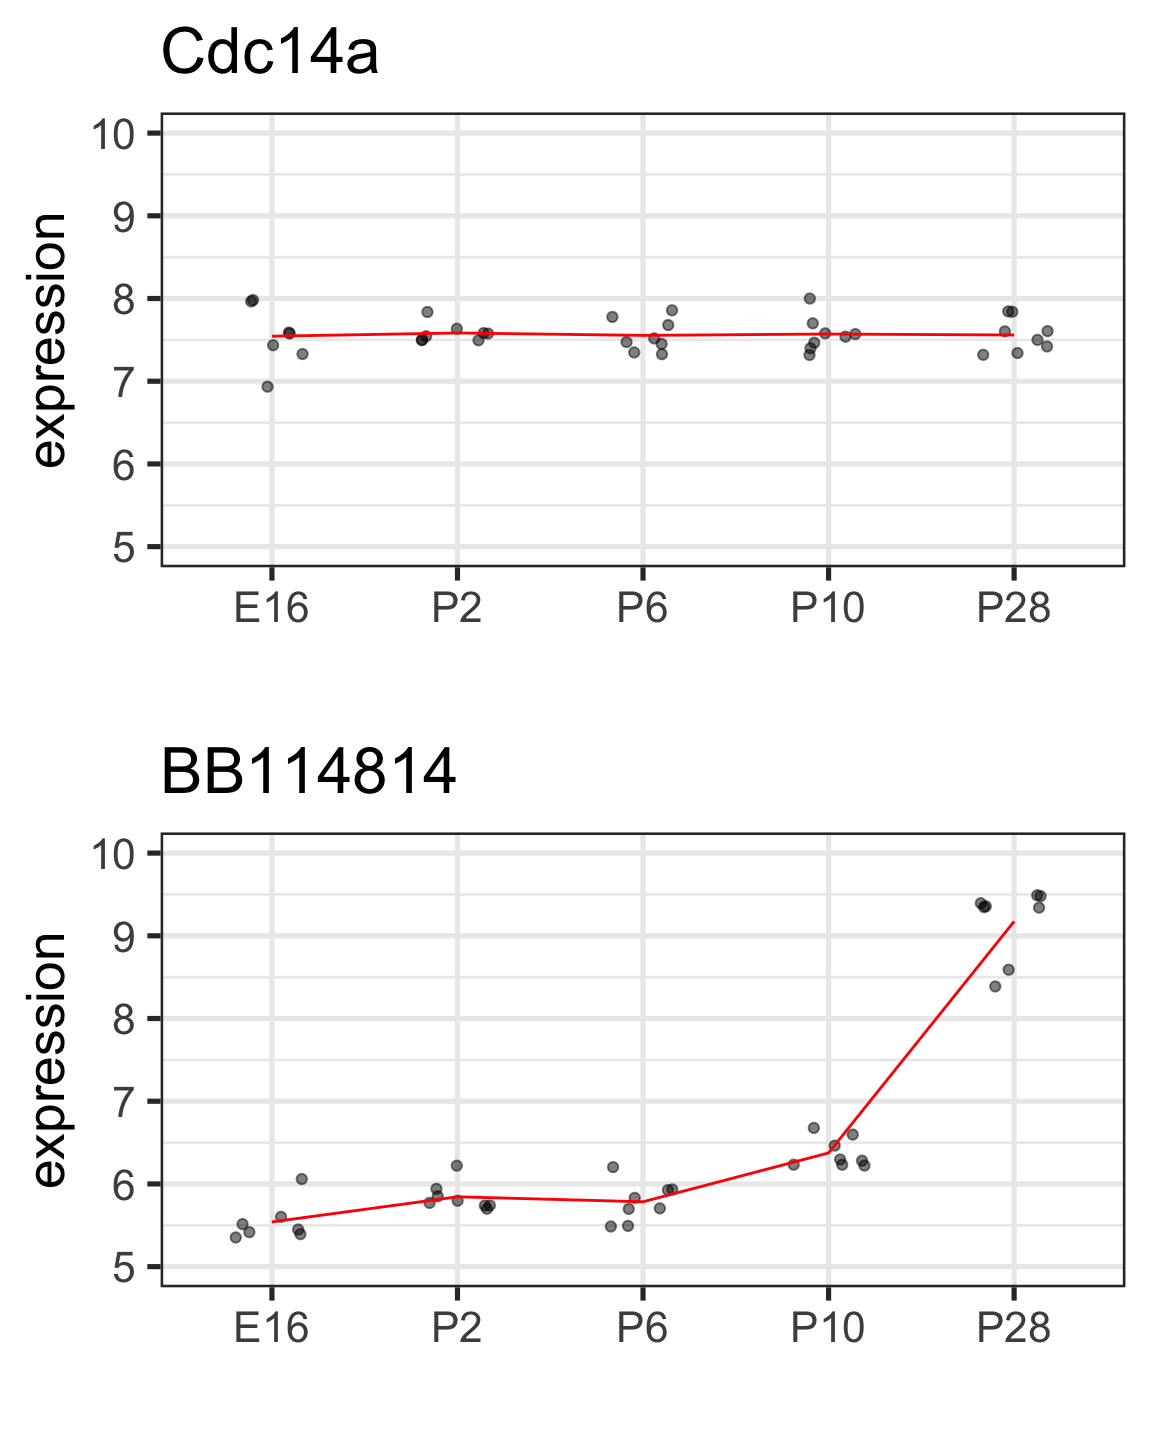
\includegraphics{Fig/supervised/unnamed-chunk-32-1} \end{center}

\normalsize
\end{frame}

\begin{frame}{Can we try out different prior (regularization)?}
\protect\hypertarget{can-we-try-out-different-prior-regularization}{}
\centerline{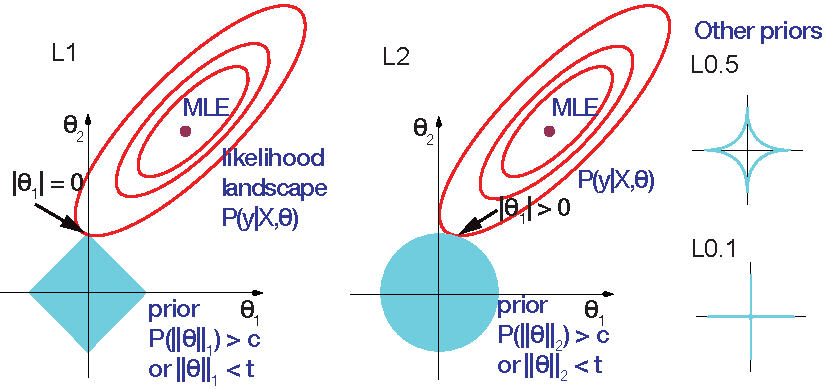
\includegraphics[width=.75\textwidth]{Vis/L1L2.pdf}}
\end{frame}

\begin{frame}{Bayesian spike-and-slab prior to achieve L0 norm}
\protect\hypertarget{bayesian-spike-and-slab-prior-to-achieve-l0-norm}{}
\centerline{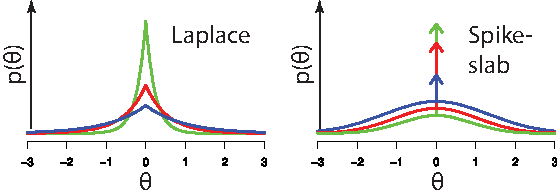
\includegraphics[width=.75\textwidth]{Vis/SS.pdf}}

\vfill

Hern'andez-Lobato \{\it et al.\} (2015)
\end{frame}

\begin{frame}{Bayesian spike-and-slab prior to select variables
(literally)}
\protect\hypertarget{bayesian-spike-and-slab-prior-to-select-variables-literally}{}
With \textbf{indicator} variables,
\({z_{1},\ldots,z_{p} \in \{0, 1\}}\), \[\left(\begin{array}{l}
y_{1}\\
y_{2}\\
\vdots\\
y_{n}
\end{array}\right)
=
z_{1} \beta_{1} \left(\begin{array}{l}
X_{11}\\
X_{21}\\
\vdots\\
X_{n1}
\end{array}\right) +
\cdots
z_{1} \beta_{p} \left(\begin{array}{l}
X_{1p}\\
X_{2p}\\
\vdots\\
X_{np}
\end{array}\right),\]
\[\mathbf{y} = X \boldsymbol{\theta} + \boldsymbol{\epsilon},\quad
\theta_{j} | z_{j} = 1 \sim \mathcal{N}\!\left(\beta_{j}, \sigma_{j}^{2}\right),\, \forall j.\]

\vfill

\flushleft{\tiny Mitchell\& Beauchamp (1988); Ishwaran\& Rao (2005); (...); Carbonetto\& Stephens (2012)}
\end{frame}

\begin{frame}{Bayesian inference with sparse Bayesian prior}
\protect\hypertarget{bayesian-inference-with-sparse-bayesian-prior}{}
\scriptsize

\normalsize

\scriptsize

\only<1>{


\begin{center}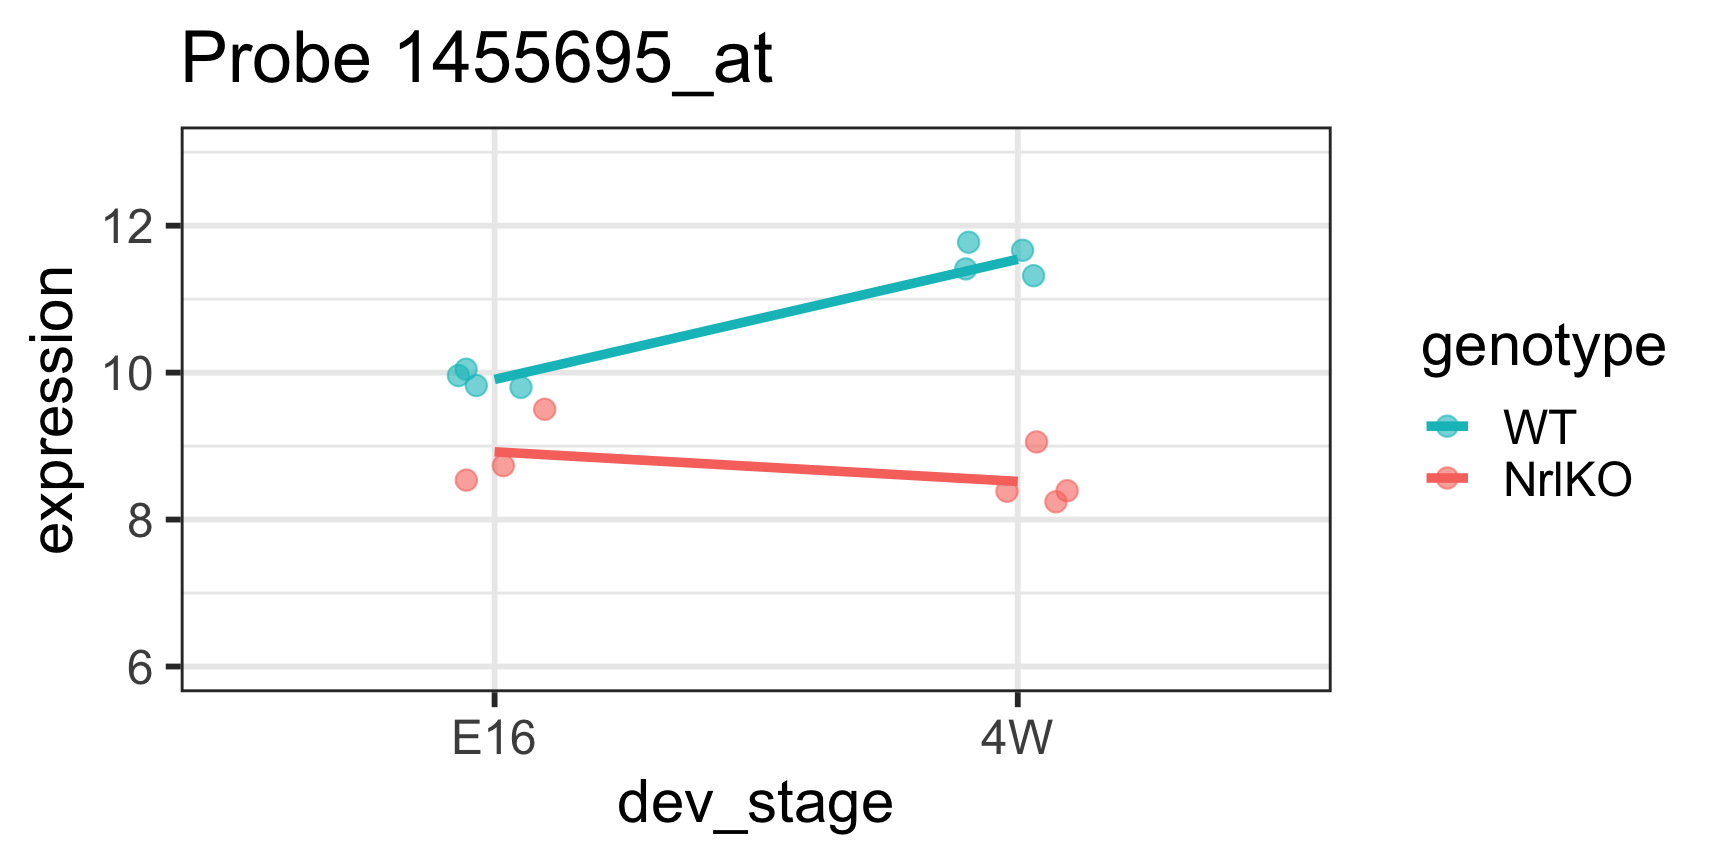
\includegraphics{Fig/supervised/unnamed-chunk-34-1} \end{center}


}

\normalsize

\scriptsize

\only<2>{


\begin{center}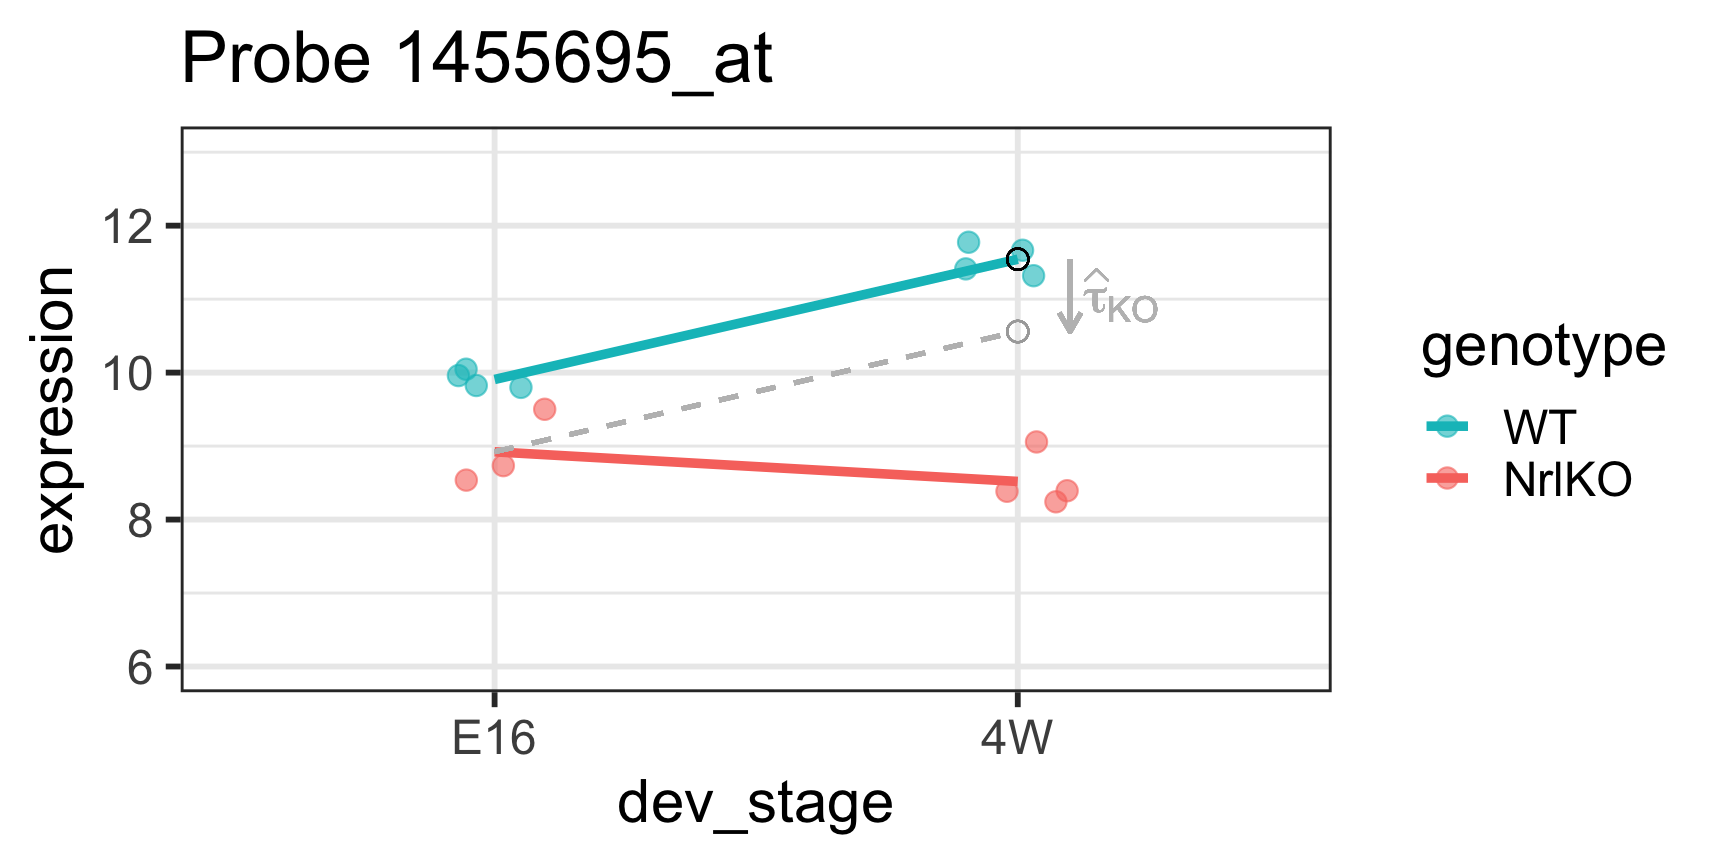
\includegraphics{Fig/supervised/unnamed-chunk-35-1} \end{center}


}

\normalsize
\end{frame}

\hypertarget{knock-off-filter-to-control-false-discovery-rate}{%
\section{Knock-off filter to control False Discovery
Rate}\label{knock-off-filter-to-control-false-discovery-rate}}

\begin{frame}{}
\protect\hypertarget{section-1}{}
\Large

Many variables to test for their non-zero-ness \(\to\)

\Huge

multiple hypothesis testing!
\end{frame}

\begin{frame}{False discovery rate in high-dimensional variable
selection}
\protect\hypertarget{false-discovery-rate-in-high-dimensional-variable-selection}{}
\Large

\[FDR(\tau) =
\frac{\sum_{j=1}^{p} I\{ |\hat{\theta}_{j}| > \tau \wedge \theta_{j} = 0 \}}
{\max\{1, \sum_{j=1}^{p} I\{ |\hat{\theta}_{j}| > \tau \} \}}\]

\normalsize

where

\begin{itemize}
\item
  \(\hat\theta_{j}\): estimation using data
\item
  \(\theta_{j}\): true random variable
\end{itemize}
\end{frame}

\begin{frame}{Can we simply attempt to control FDR as in DEG analysis?}
\protect\hypertarget{can-we-simply-attempt-to-control-fdr-as-in-deg-analysis}{}
\Large

\begin{enumerate}
\item
  Perform variable-by-variable association tests
\item
  Combine p-values
\item
  Run multiple hypothesis correction (e.g., Bonferroni,
  Benjamini-Hochberg)
\end{enumerate}
\end{frame}

\begin{frame}{Can we simply attempt to control FDR as in DEG analysis?}
\protect\hypertarget{can-we-simply-attempt-to-control-fdr-as-in-deg-analysis-1}{}
\scriptsize

\normalsize

\scriptsize

\only<1>{


\begin{center}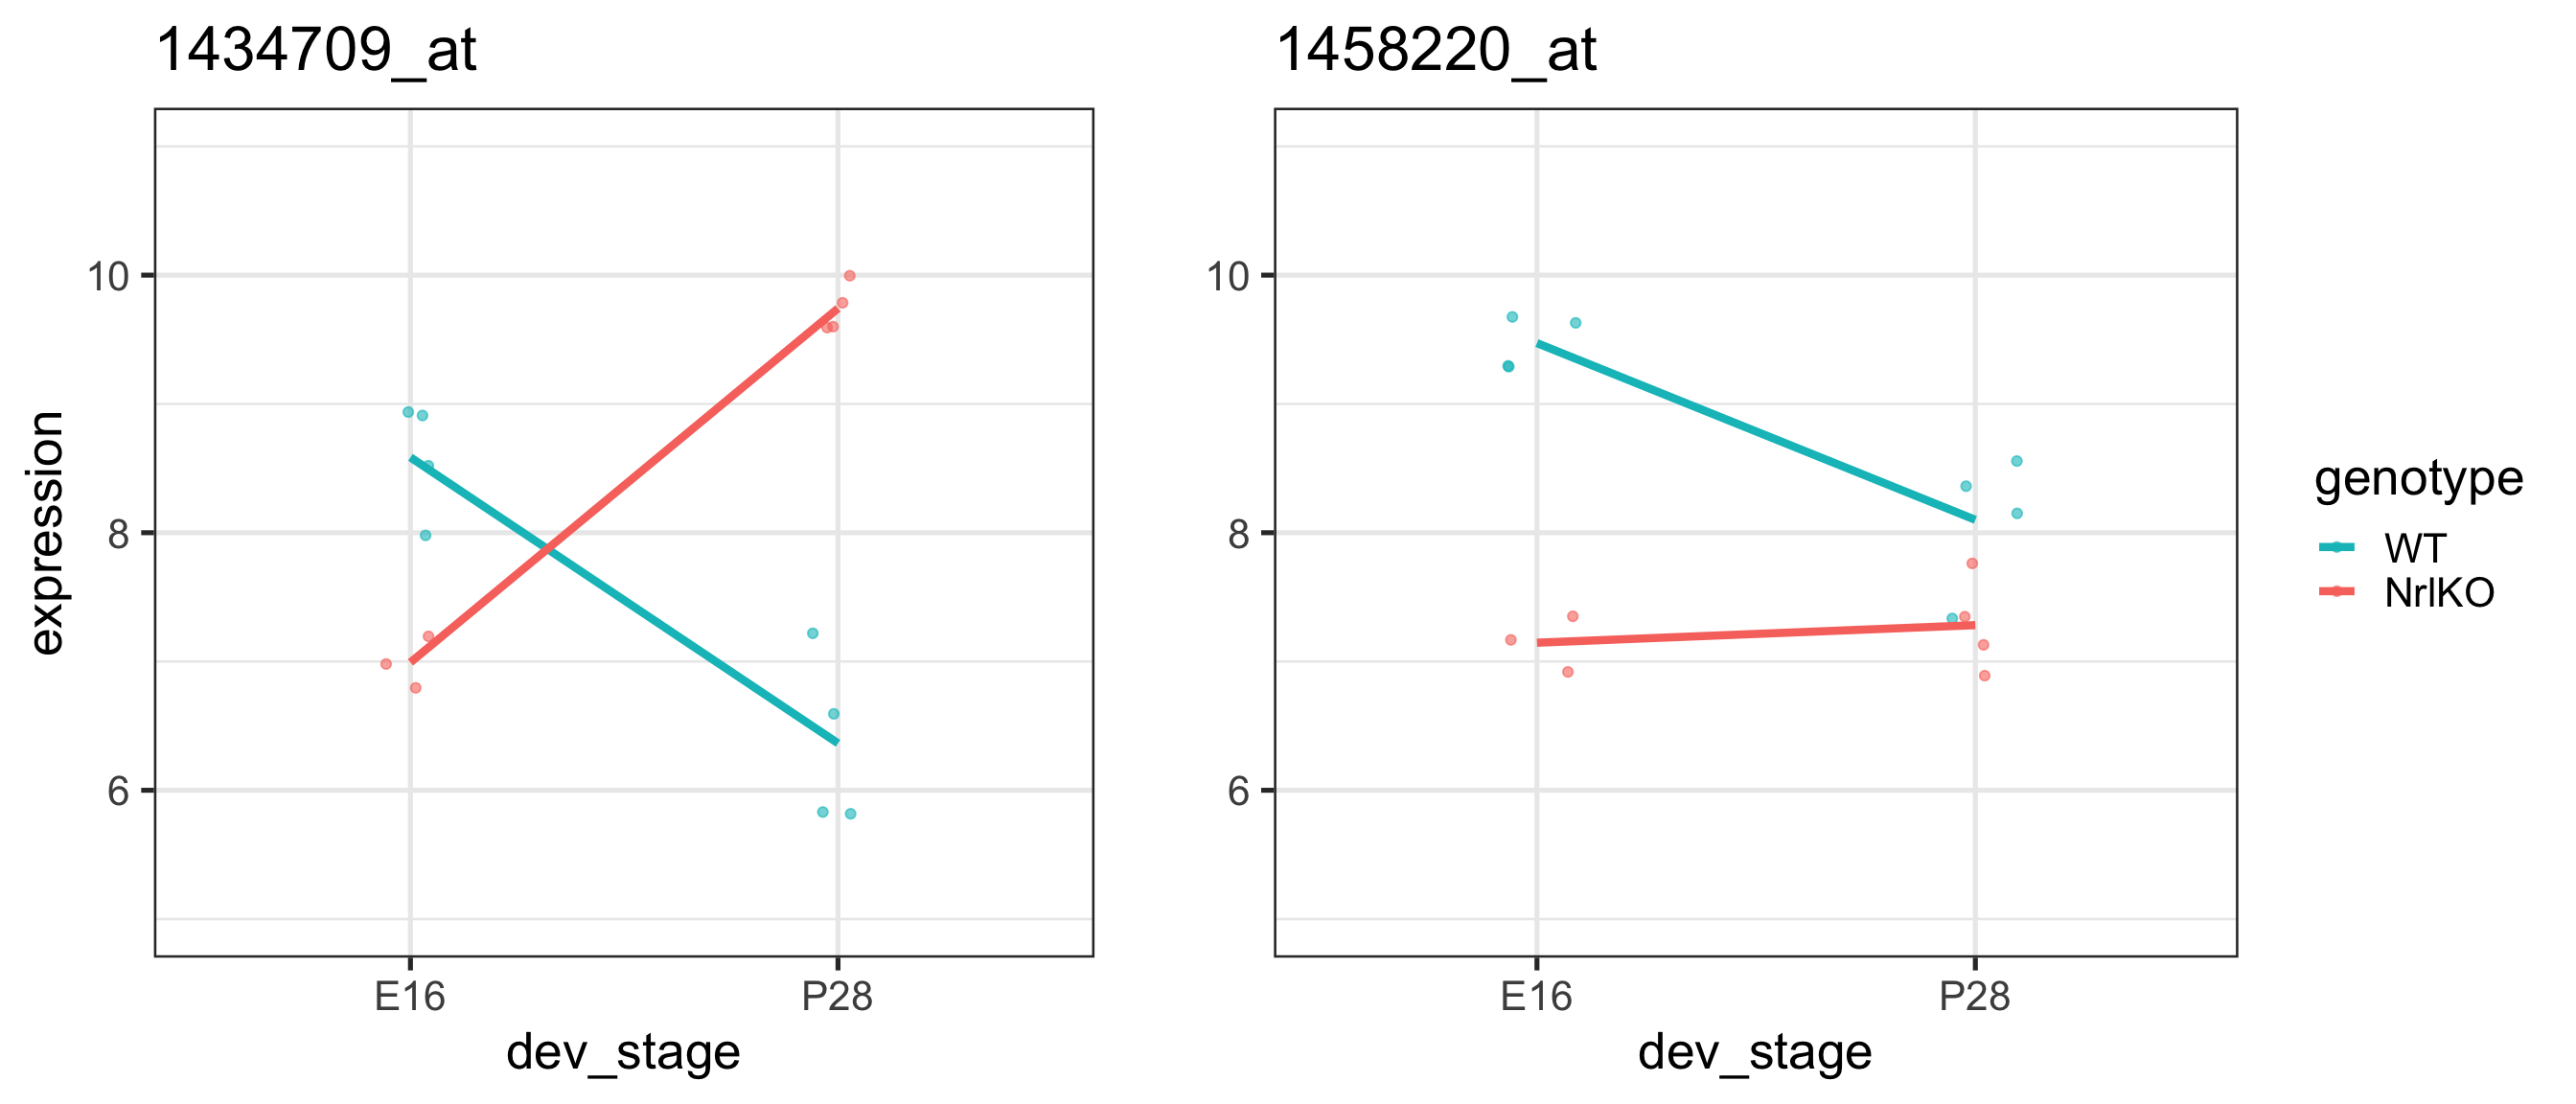
\includegraphics{Fig/supervised/unnamed-chunk-37-1} \end{center}


}

\normalsize

\scriptsize

\only<2>{


\begin{center}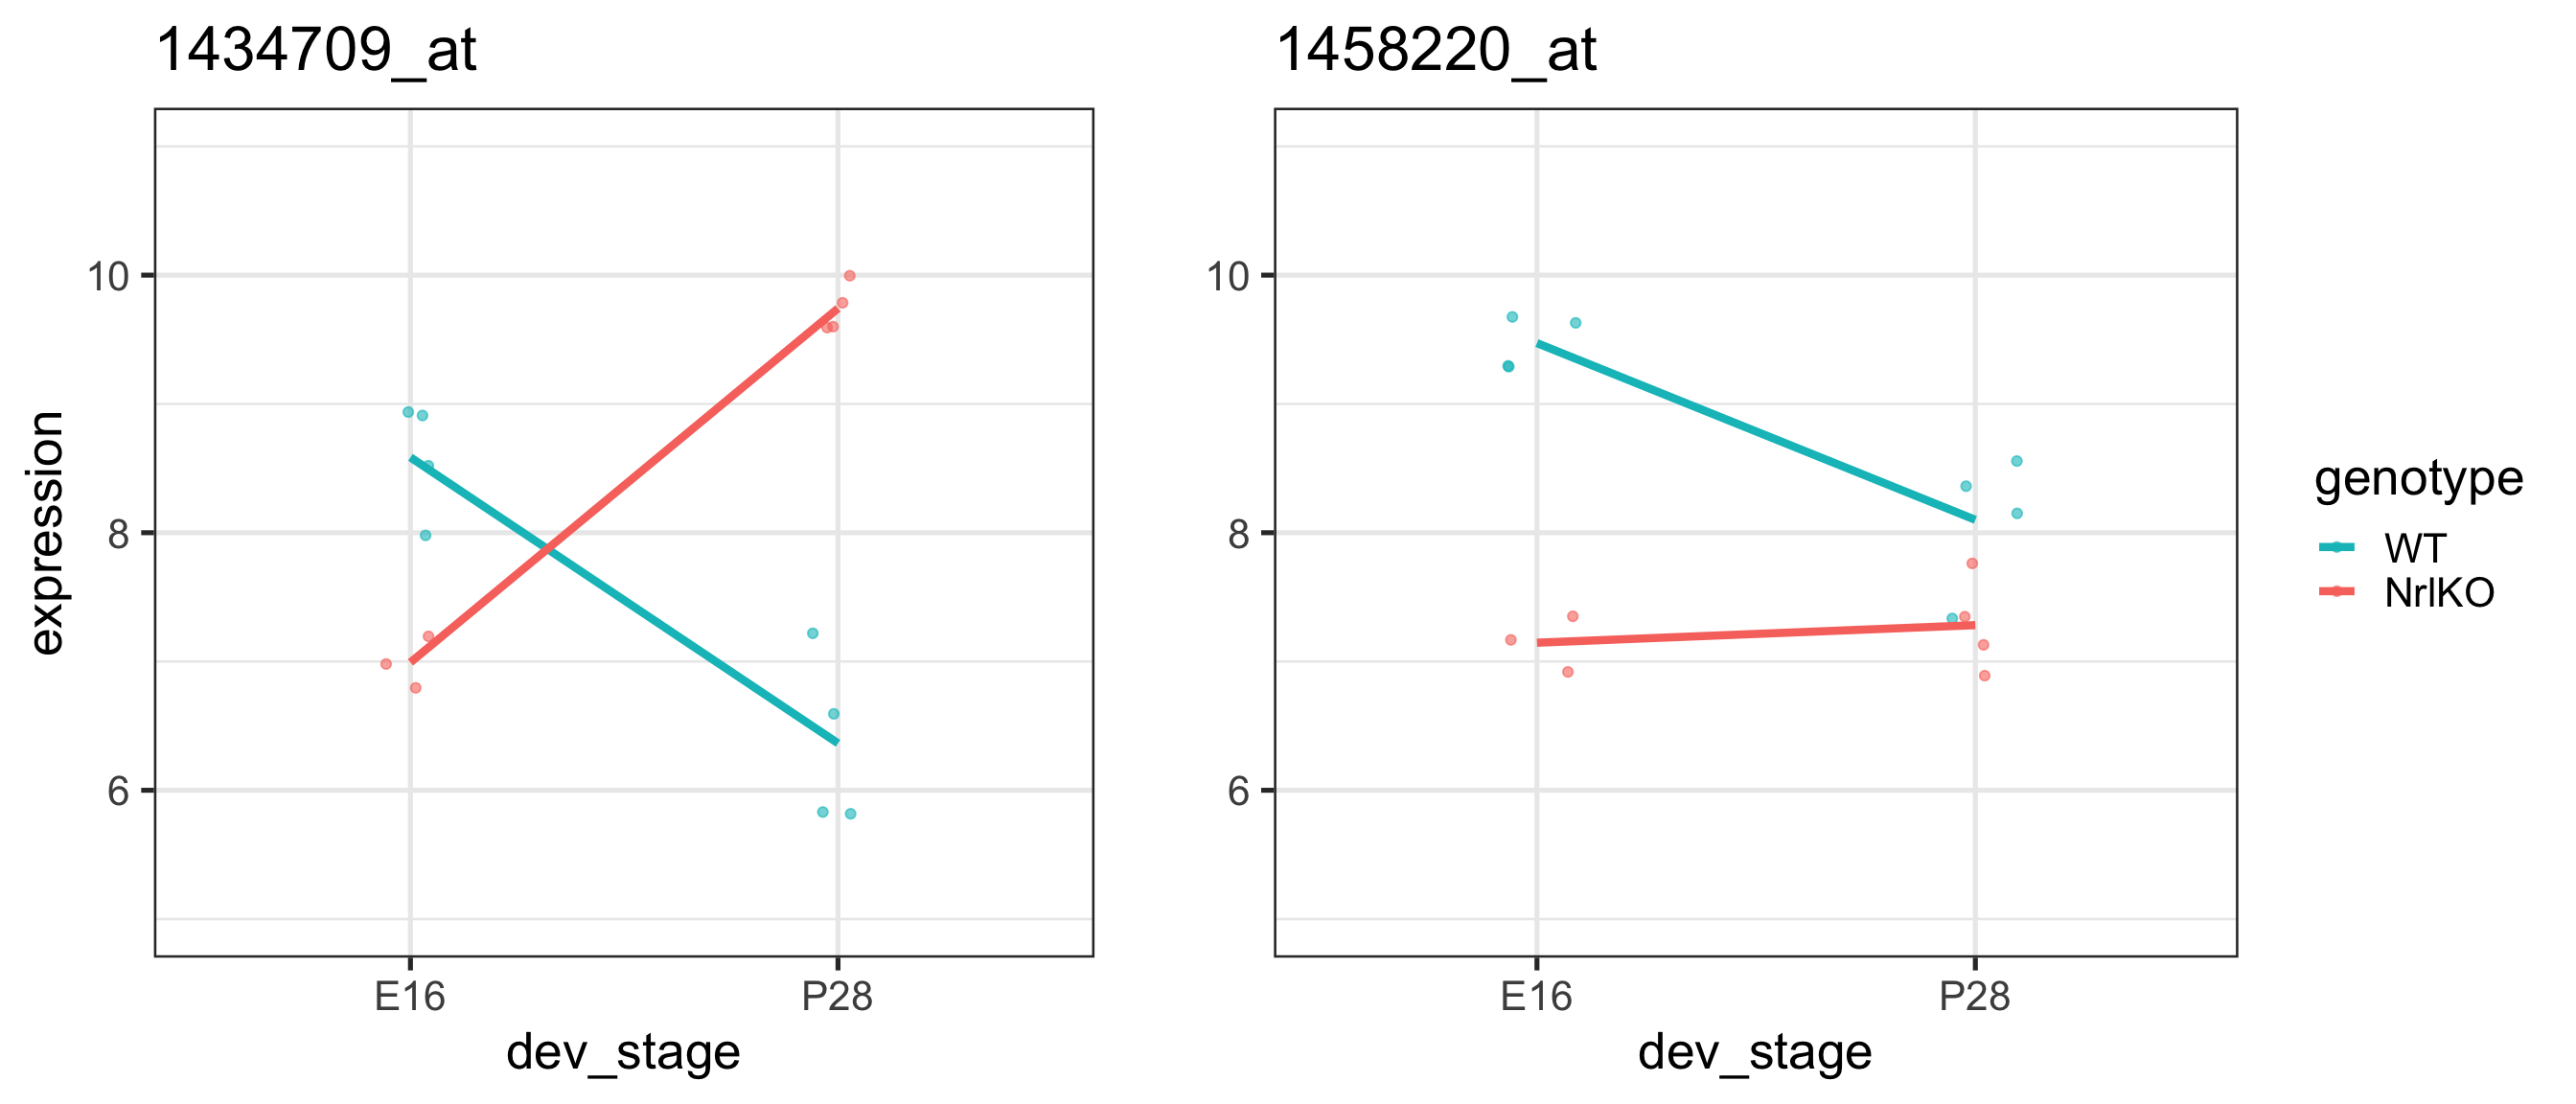
\includegraphics{Fig/supervised/unnamed-chunk-38-1} \end{center}


}

\normalsize

Variant-by-variant tests fail to control false discovery rate. Why?
\end{frame}

\begin{frame}{How about using multivariate OLS results?}
\protect\hypertarget{how-about-using-multivariate-ols-results}{}
\scriptsize

\begin{center}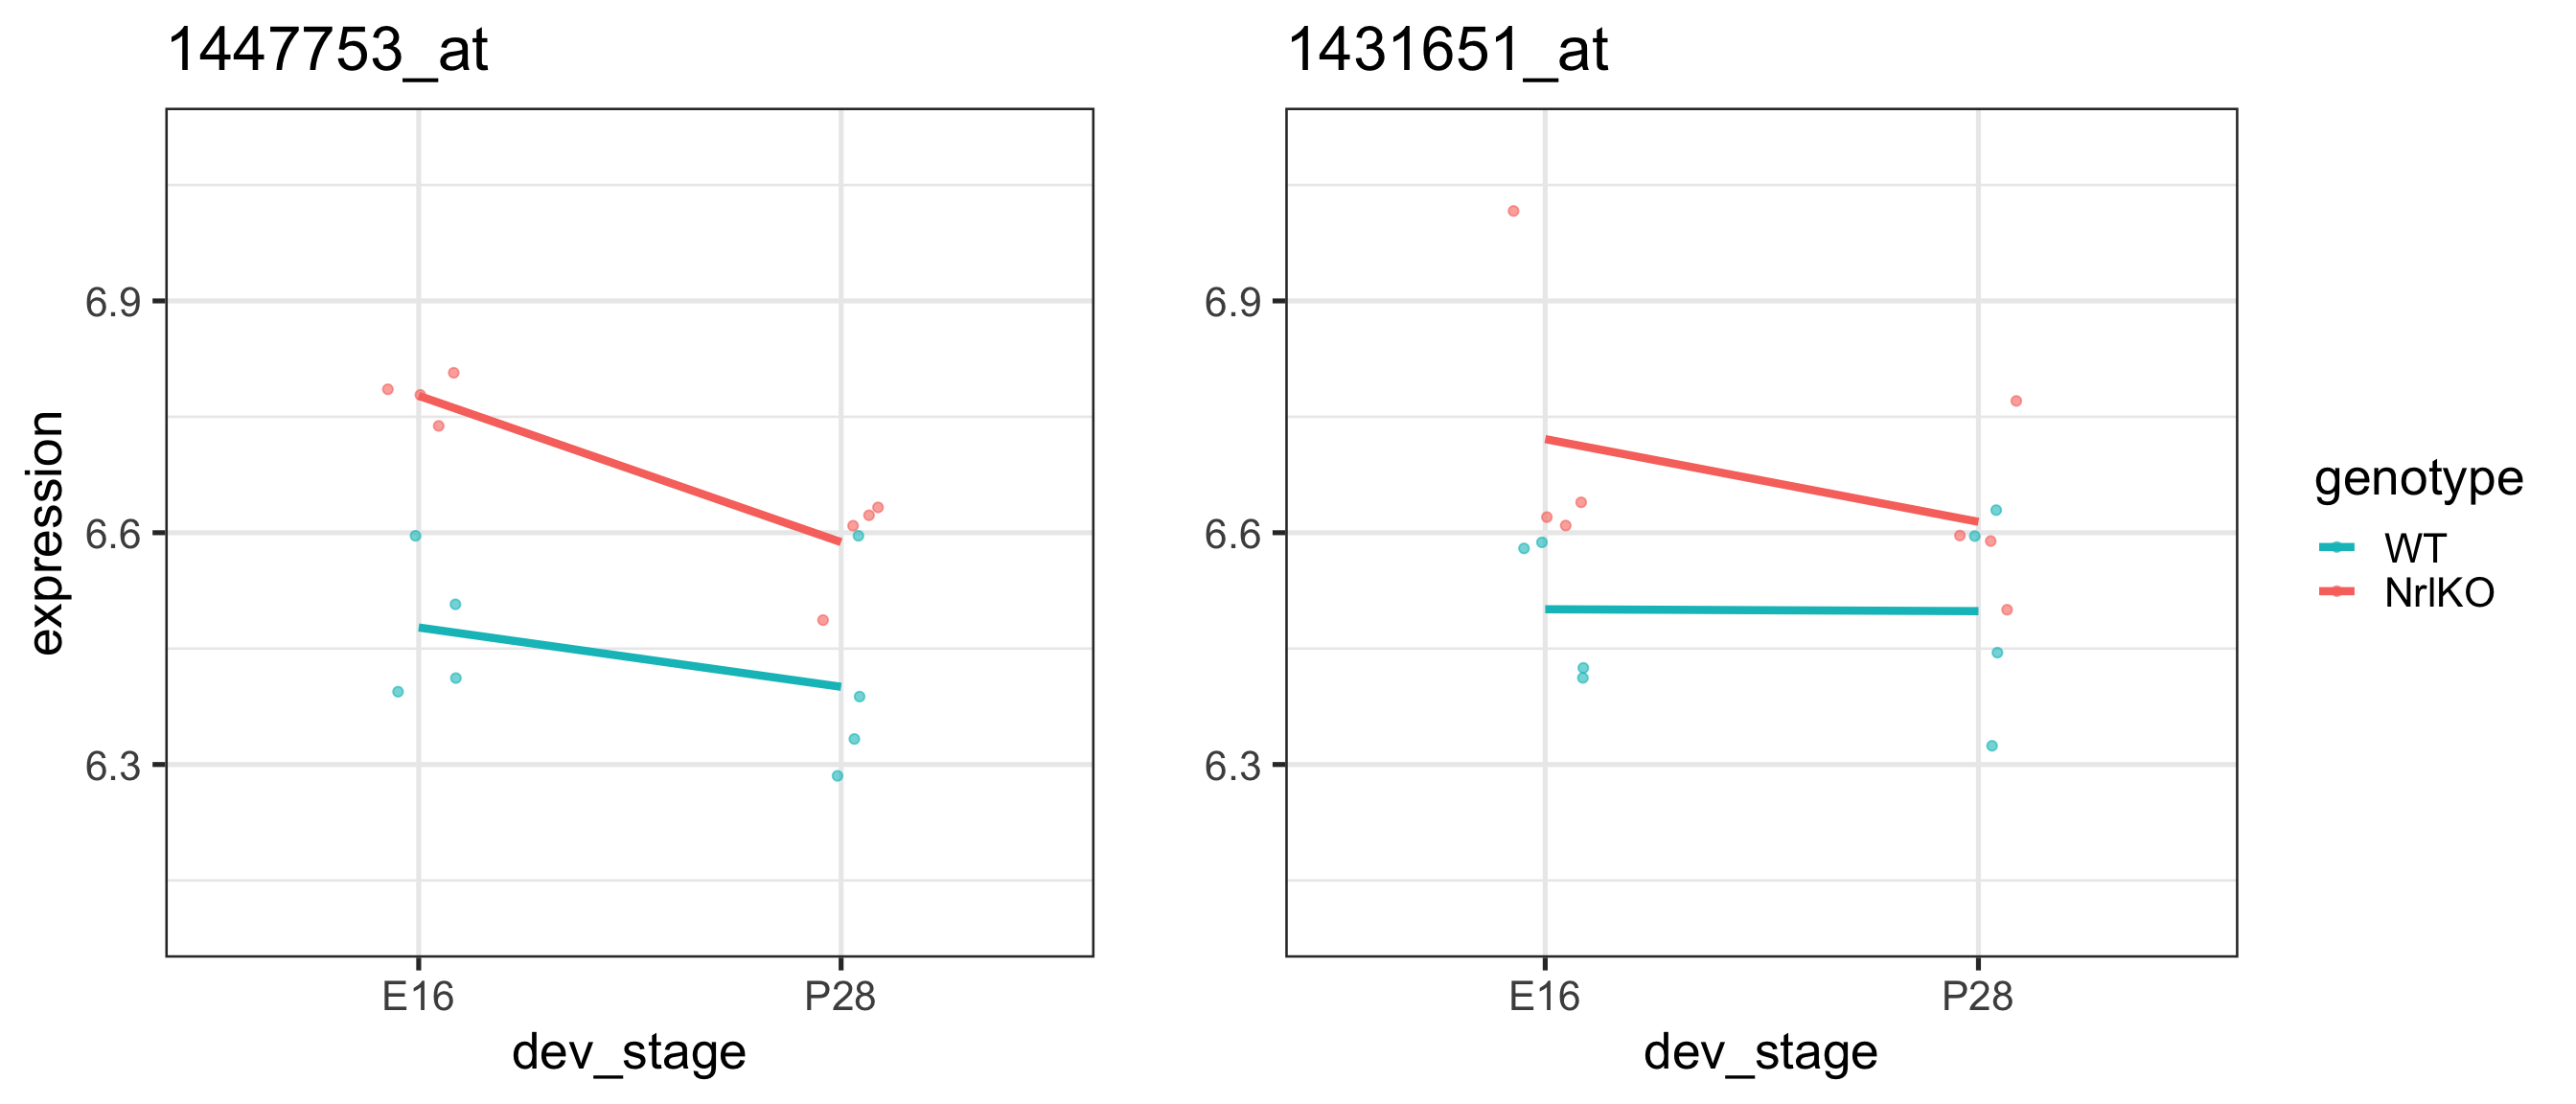
\includegraphics{Fig/supervised/unnamed-chunk-39-1} \end{center}

\normalsize

\begin{itemize}
\tightlist
\item
  What happened to the other 1000 variables?
\end{itemize}
\end{frame}

\begin{frame}{Bayesian posterior inclusion probability can help}
\protect\hypertarget{bayesian-posterior-inclusion-probability-can-help}{}
\scriptsize

\normalsize

\scriptsize

\begin{center}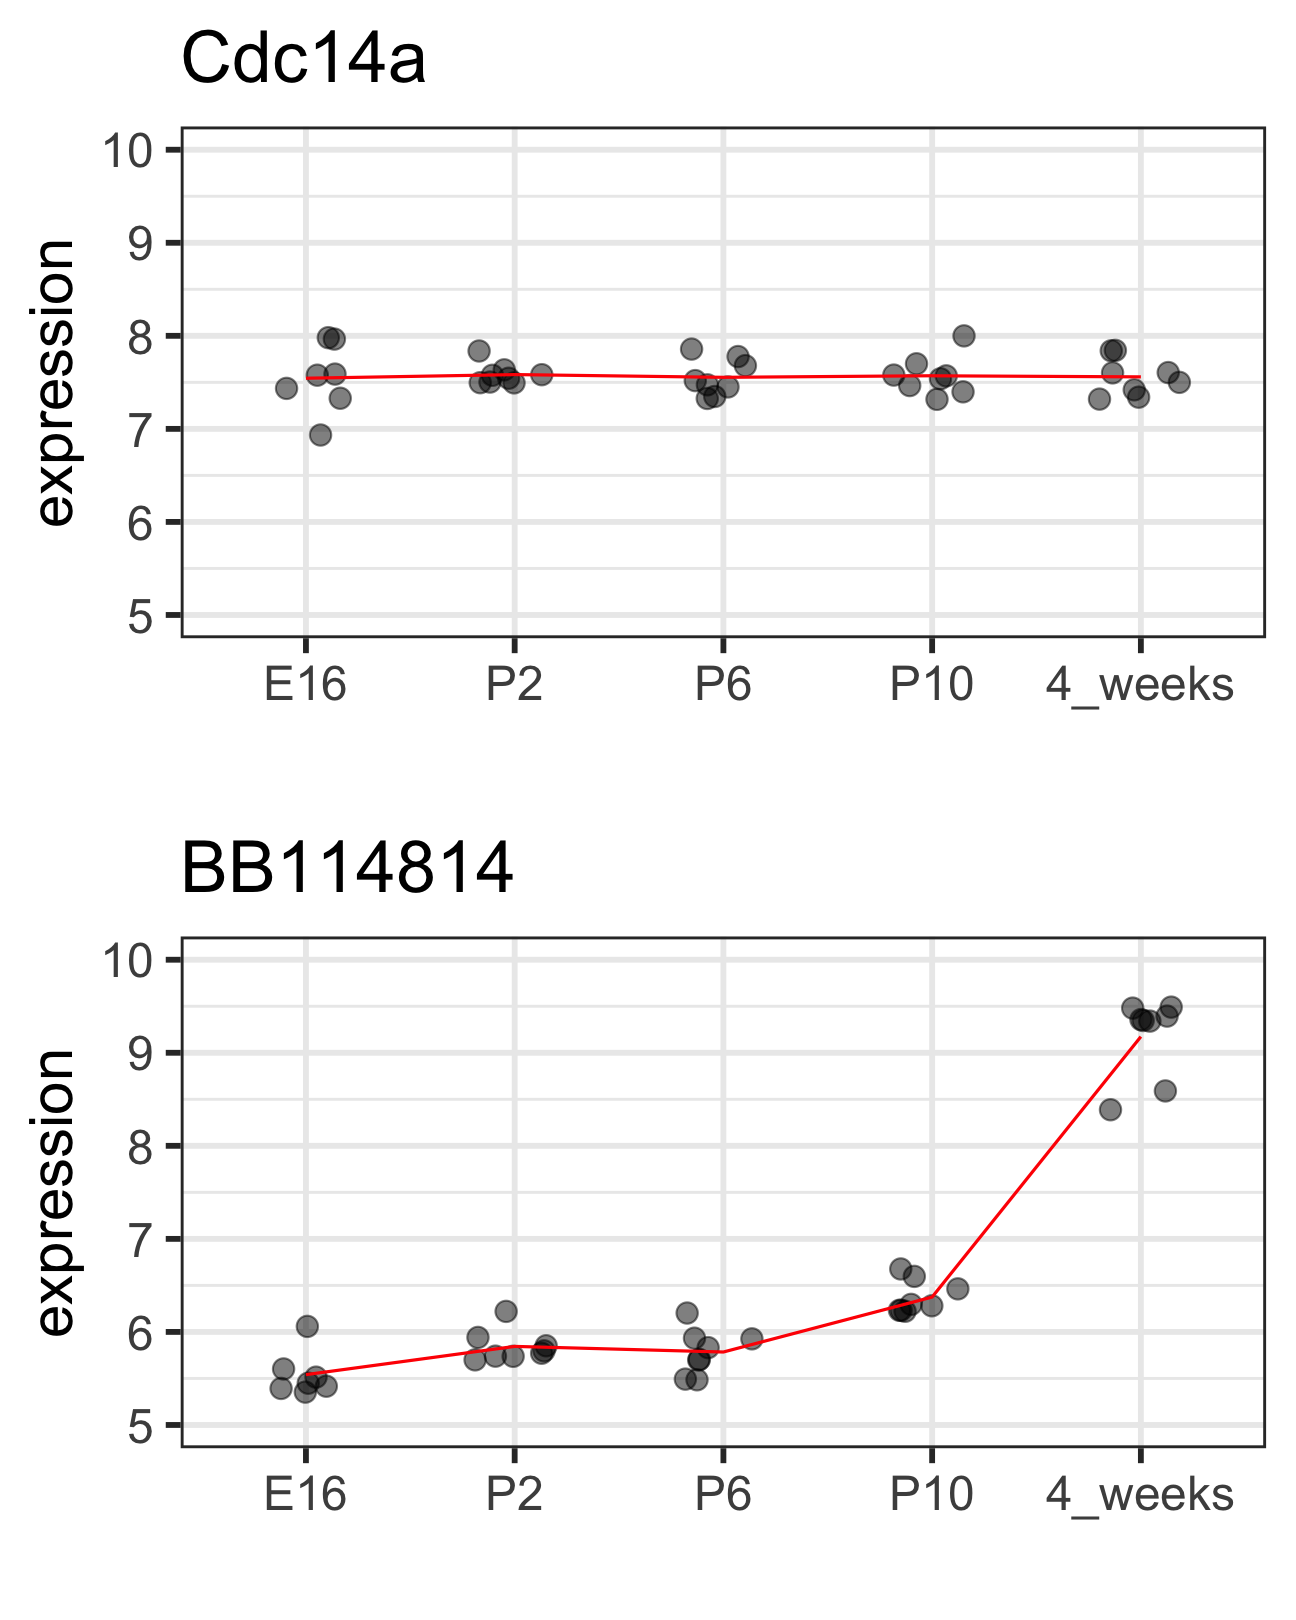
\includegraphics{Fig/supervised/unnamed-chunk-41-1} \end{center}

\normalsize

\begin{itemize}
\tightlist
\item
  Okay, but what is FDR? Can we consider (\(1-\) PIP) as FDR?
\end{itemize}
\end{frame}

\begin{frame}[fragile]{How we estimate the False Discovery Rate for
non-zero regression coefficient?}
\protect\hypertarget{how-we-estimate-the-false-discovery-rate-for-non-zero-regression-coefficient}{}
\Large

\begin{itemize}
\item
  What should be the null distribution of regression coefficient?
\item
  Is it t-distributed (the default option of \texttt{lm})?
\end{itemize}
\end{frame}

\begin{frame}[fragile]{First attempt: Construct ``null'' regression data
by sample permutation?}
\protect\hypertarget{first-attempt-construct-null-regression-data-by-sample-permutation}{}
\large

\begin{Shaded}
\begin{Highlighting}[]
\FunctionTok{set.seed}\NormalTok{(}\DecValTok{17}\NormalTok{)}
\NormalTok{X.perm }\OtherTok{\textless{}{-}} \FunctionTok{apply}\NormalTok{(X, }\DecValTok{2}\NormalTok{, sample)}
\end{Highlighting}
\end{Shaded}

\normalsize

\scriptsize

\normalsize

\Large

\begin{itemize}
\item
  What are we missing?
\item
  It is not clear whether we can control Type-I error.
\end{itemize}

\[\mathbf{y} \sim [X, \underbrace{\tilde{X}}_{\textsf{\color{red} permuted}}]\]
\end{frame}

\begin{frame}{Can we learn FDR cutoff from the permuted coefficients?}
\protect\hypertarget{can-we-learn-fdr-cutoff-from-the-permuted-coefficients}{}
\scriptsize

\normalsize

\scriptsize

\only<1>{


\begin{center}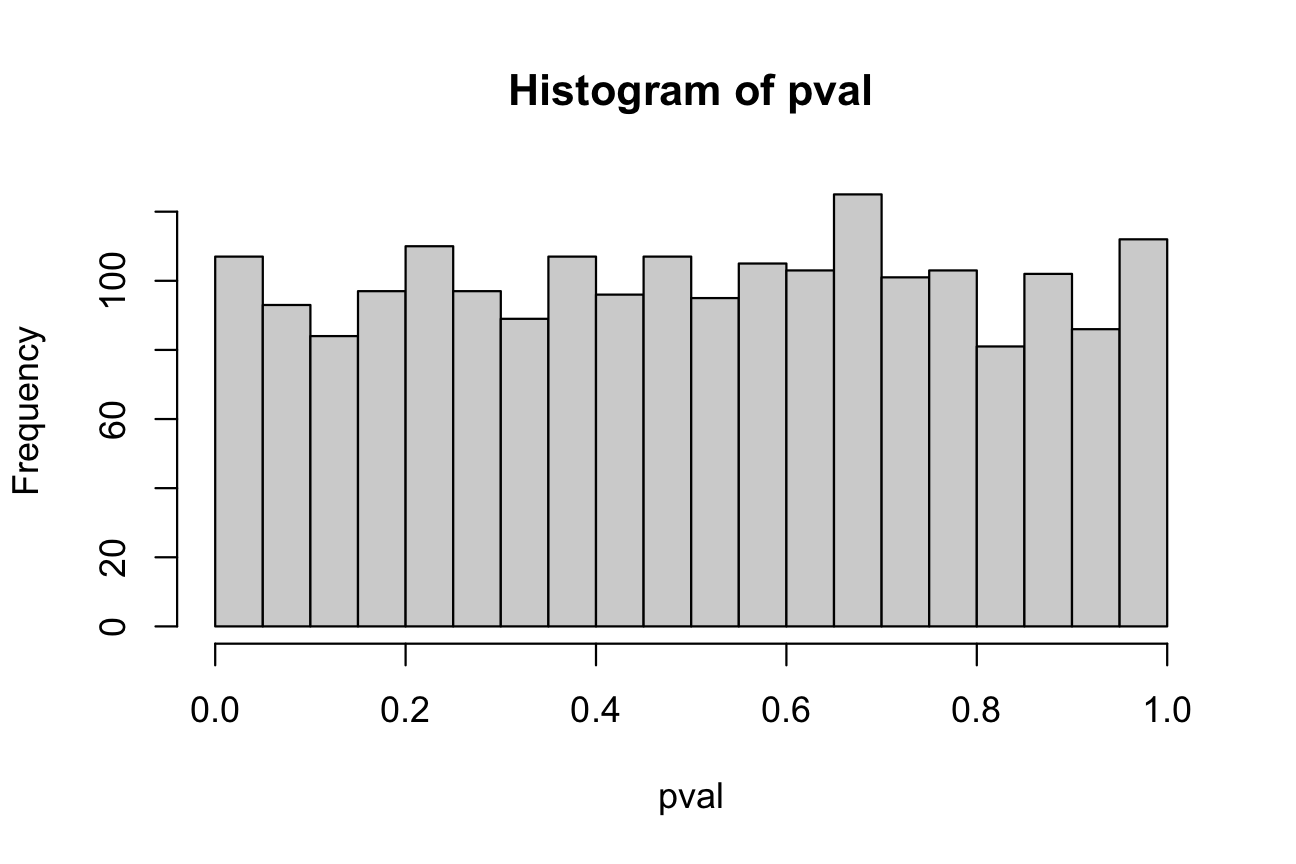
\includegraphics{Fig/supervised/unnamed-chunk-45-1} \end{center}


}

\normalsize

\scriptsize

\only<2>{


\begin{center}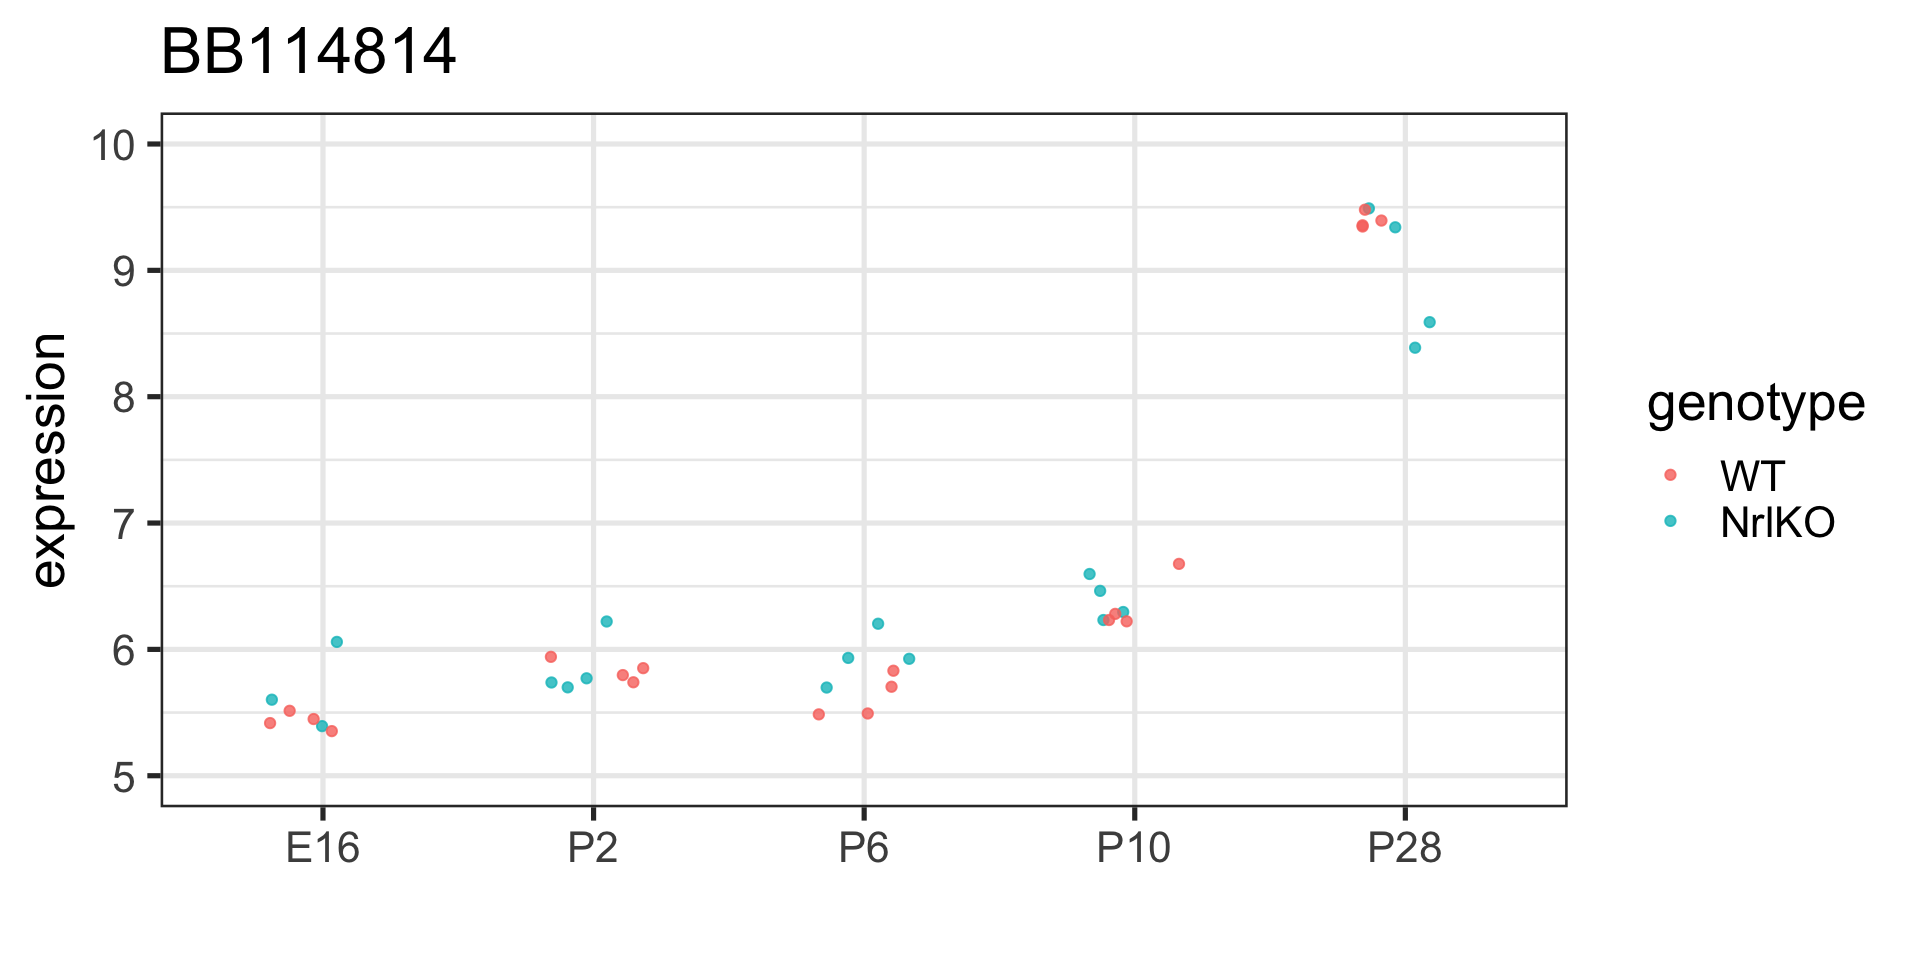
\includegraphics{Fig/supervised/unnamed-chunk-46-1} \end{center}


}

\normalsize
\end{frame}

\begin{frame}{Can we calibrate FDR using the permuted data?}
\protect\hypertarget{can-we-calibrate-fdr-using-the-permuted-data}{}
\large

Not really\ldots{}

\begin{itemize}
\item
  Let \(\rho_{j}\) be estimated posterior probability
  \(p(\theta_{j} \neq 0|\textsf{data})\)
\item
  empirical False Discovery Rate =
\end{itemize}

\[\frac{\sum_{j} I\{\rho_{j} > \tau \wedge \theta_{j} = 0 \}}{\sum_{j} I\{ \rho_{j} > \tau \}}\]

\scriptsize

\normalsize

In this example, we have 93 \%

\begin{itemize}
\tightlist
\item
  What have we missed?
\end{itemize}
\end{frame}

\begin{frame}{What went wrong?}
\protect\hypertarget{what-went-wrong}{}
\Large

\begin{enumerate}
\item
  We need to apply different threshold levels for different varaibles
\item
  We didn't consider correlation (col-linearity) structures between
  variables
\item
  Naive permutation steps break the covariance structure in \(X\)
\end{enumerate}
\end{frame}

\begin{frame}{Construct valid ``null'' matrix preserving correlation
structures}
\protect\hypertarget{construct-valid-null-matrix-preserving-correlation-structures}{}
\begin{block}{Knock-off filter}
\protect\hypertarget{knock-off-filter}{}
Given \(X = (X_{1},\ldots, X_{p})\), a new family of random variables,
\(\tilde{X} = (\tilde{X}_{1},\ldots, \tilde{X}_{p})\) are considered a
valid ``knockoff'' filter if

\begin{enumerate}
\item
  \(\tilde{X}\) is independent of \(Y\) given \(X\)
\item
  distribution of \((X, \tilde{X})\) remain invariant to any swapping
  between the original and knockoff variables.
\end{enumerate}
\end{block}

E.g.,

\onslide<2->{
\centering
    $(X_{1},{\color{red} X_{2}},X_{3}, \tilde{X}_{1}, {\color{red} \tilde{X}_{2}},\tilde{X}_{3}) \overset{d}{=}
      (X_{1},{\color{red} \tilde{X}_{2}}, X_{3}, \tilde{X}_{1}, {\color{red} X_{2}},\tilde{X}_{3})$
}
\onslide<3>{
\centering
    $({\color{red} X_{1}, X_{2}}, X_{3}, {\color{red}\tilde{X}_{1}, \tilde{X}_{2}}, \tilde{X}_{3}) \overset{d}{=}
      ({\color{red} \tilde{X}_{1}, \tilde{X}_{2}}, X_{3}, {\color{red} X_{1}, X_{2}}, \tilde{X}_{3})$
\centerline{(...)}
}

\vfill

\tiny

Candes, Fan, Janson, and Lv, \emph{Panning for Gold: Model-X Knockoffs
for High-dimensional Controlled Variable Selection}, (2018)
\end{frame}

\begin{frame}{}
\protect\hypertarget{section-2}{}
\end{frame}

\begin{frame}{A reasonable approximation for knockoff construction}
\protect\hypertarget{a-reasonable-approximation-for-knockoff-construction}{}
\Large
\begin{enumerate}
\item<1-> Fit $X \sim W Z$ matrix factorization
\item<2-> Predict $\hat{X} \gets \hat{U} \hat{Z}$
\item<3-> Take residuals $\epsilon = X - \hat{X}$
\item<4-> Add permute residuals $\tilde{\epsilon}$, i.e., $\tilde{X} = \hat{X} + \tilde{\epsilon}$
\end{enumerate}

\vfill

\tiny

Zhu \emph{et al.} DeepLINK: Deep learning inference using knockoffs with
applications to genomics (2021)
\end{frame}

\begin{frame}{Knockoff statistics}
\protect\hypertarget{knockoff-statistics}{}
\large

\[\mathbf{y} \sim [X, \underset{\textsf{\color{red} knockoff}}{\tilde{X}}]\]

For each variable \(j\) (Lasso):

\[W_{j} = |\hat{\theta}_{j}| - |\tilde{\theta}_{j}|\]

For each variable \(j\) (Bayesian PIP):

\[W_{j} = \hat{\rho}_{j} - \tilde{\rho}_{j}\]
\end{frame}

\begin{frame}{Knockoff statistics: What is FDR here?}
\protect\hypertarget{knockoff-statistics-what-is-fdr-here}{}
\scriptsize

\normalsize

\scriptsize

\normalsize

\scriptsize

\only<1>{


\begin{center}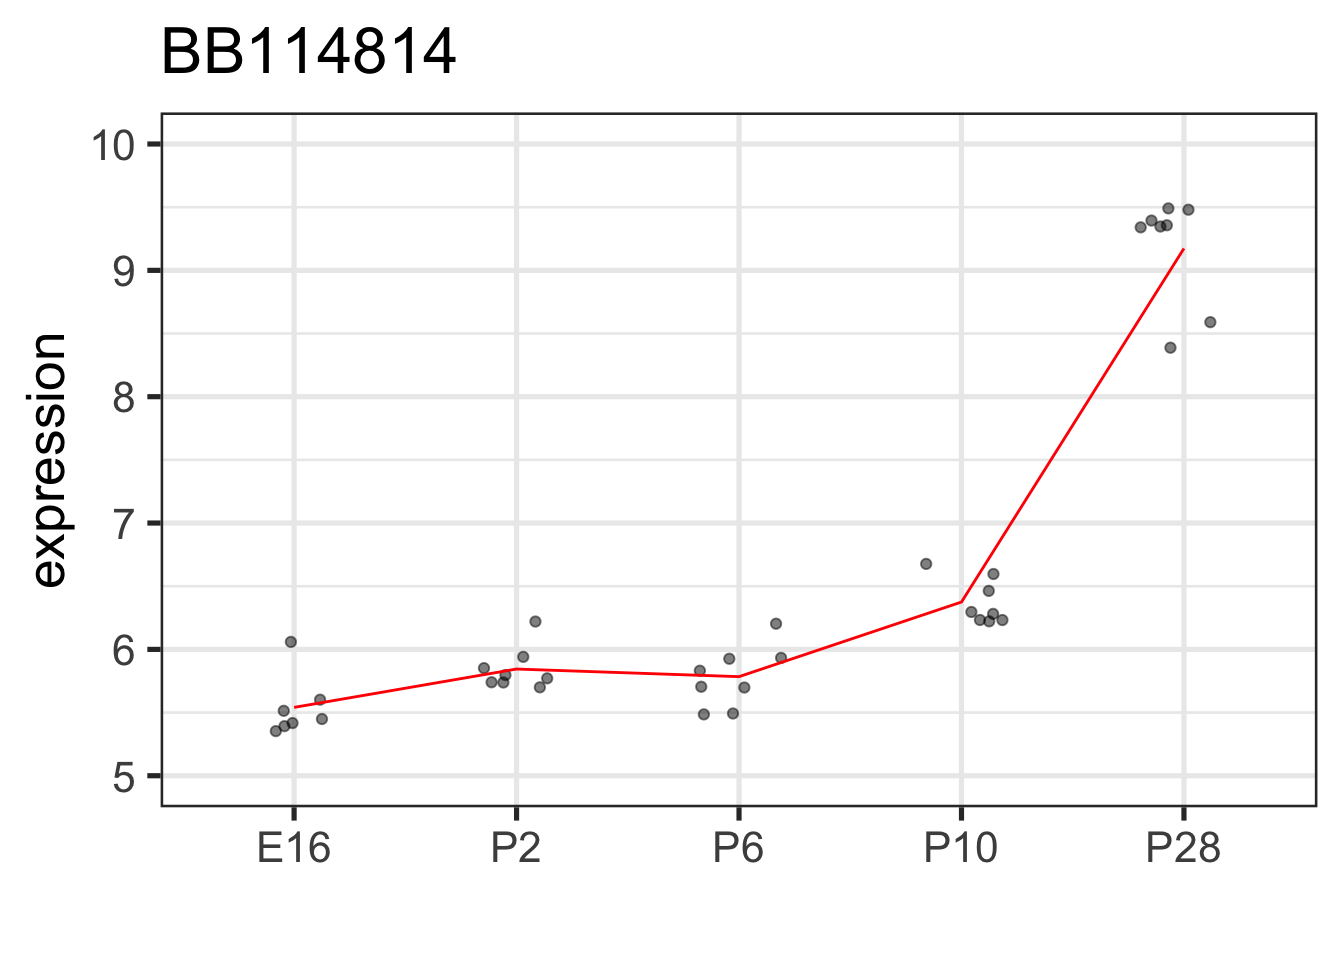
\includegraphics{Fig/supervised/unnamed-chunk-50-1} \end{center}


}

\normalsize

\scriptsize

\only<2>{


\begin{center}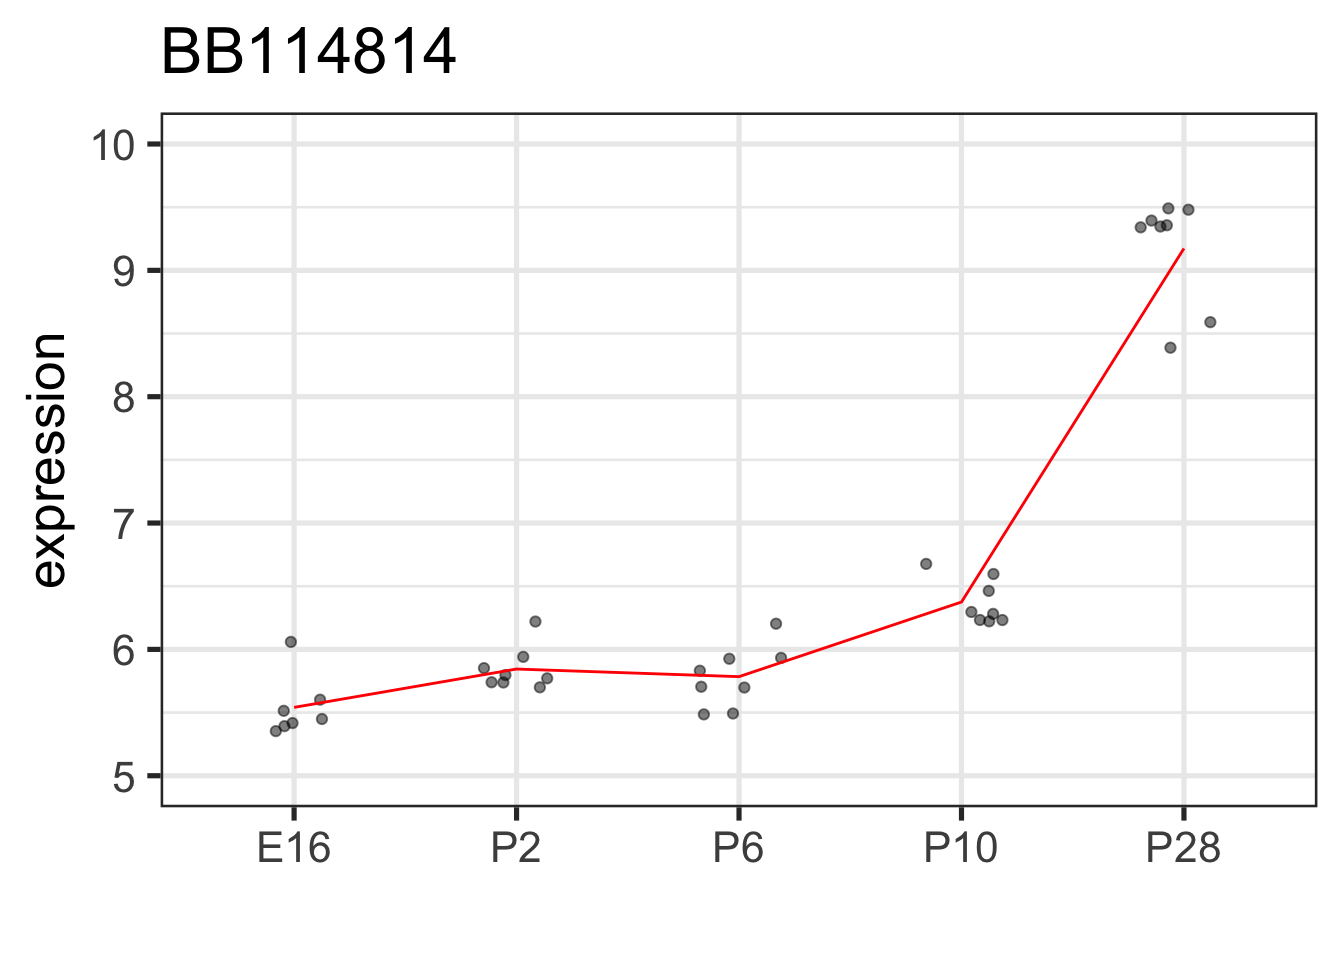
\includegraphics{Fig/supervised/unnamed-chunk-51-1} \end{center}


}

\normalsize
\end{frame}

\hypertarget{bias-variance-tradeoff}{%
\section{Bias-variance tradeoff}\label{bias-variance-tradeoff}}

\begin{frame}{What is a good classifier?}
\protect\hypertarget{what-is-a-good-classifier}{}
\scriptsize

\only<1>{


\begin{center}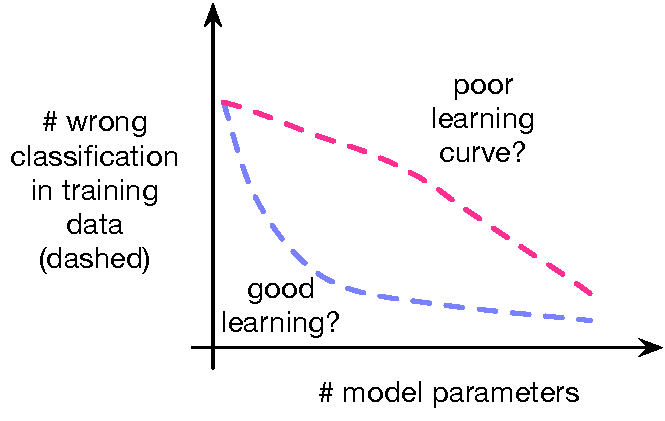
\includegraphics[height=.6\textheight]{Vis/supervised_learning_curves} \end{center}


}

\normalsize

\scriptsize

\only<2>{


\begin{center}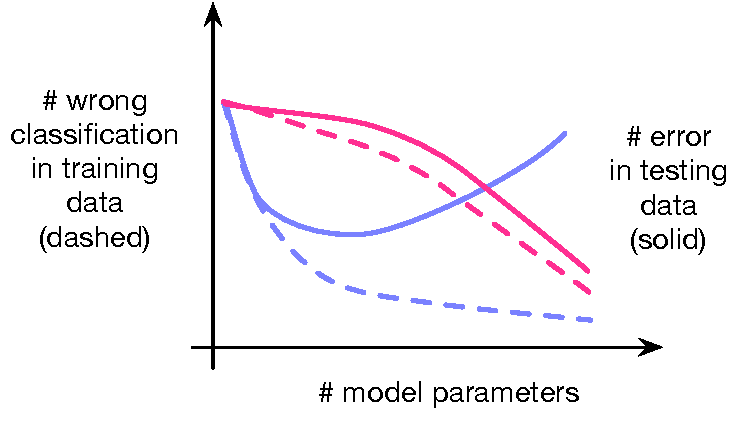
\includegraphics[height=.6\textheight]{Vis/supervised_learning_curves_2} \end{center}


}

\normalsize

\scriptsize

\only<3>{


\begin{center}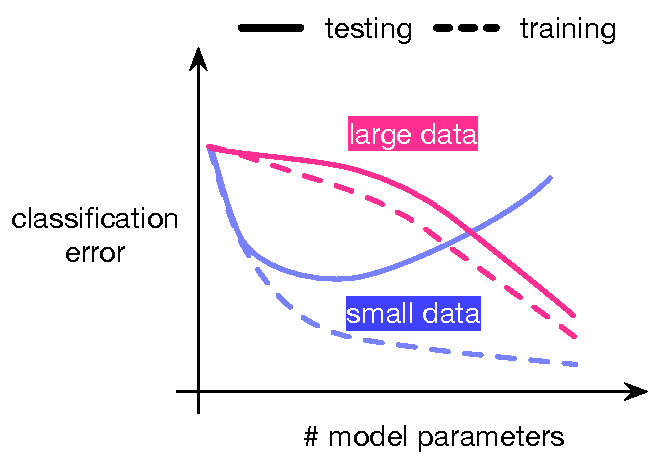
\includegraphics[height=.7\textheight]{Vis/supervised_learning_curves_3} \end{center}


}

\normalsize
\end{frame}

\begin{frame}{How do we know if one classier is better than the other?}
\protect\hypertarget{how-do-we-know-if-one-classier-is-better-than-the-other}{}
\large

\begin{itemize}
\item
  Training vs.~(unseen) testing data
\item
  Our hope: training \(\approx\) testing
\end{itemize}
\end{frame}

\begin{frame}{The ultimate goal: generalization error minimization}
\protect\hypertarget{the-ultimate-goal-generalization-error-minimization}{}
\Large

k-fold CV error \(\to\) leave-one-out CV error \(\to\) generalization
error

\vfill

\normalsize

\begin{itemize}
\item
  No matter what may come, we will still predict as good as this\ldots{}
\item
  We will use k-fold cross validation error to estimate generalization
  error
\end{itemize}
\end{frame}

\begin{frame}{Bias-variance tradeoff explains why a regularized
regression works in practice}
\protect\hypertarget{bias-variance-tradeoff-explains-why-a-regularized-regression-works-in-practice}{}
\large

\[
\min_{\boldsymbol{\theta}} \quad
\overbrace{(\mathbf{y} - X\boldsymbol{\theta})^{\top}(\mathbf{y} - X\boldsymbol{\theta})}^{\textsf{\color{blue} bias}} + \underbrace{\lambda \alpha \|\boldsymbol{\theta}\|_{1}}_{\textsf{\color{red} variable selection}} + \underbrace{\lambda (1 - \alpha) \|\boldsymbol{\theta}\|_{2}}_{\textsf{\color{magenta} shrinkage}}
\]

\begin{itemize}
\tightlist
\item
  The second and the third terms control the model variance
\end{itemize}
\end{frame}

\hypertarget{discussion}{%
\section{Discussion}\label{discussion}}

\begin{frame}{Other methods that we haven't had a chance to discuss}
\protect\hypertarget{other-methods-that-we-havent-had-a-chance-to-discuss}{}
\begin{itemize}
\item
  Ensemble learning

  \begin{itemize}
  \tightlist
  \item
    Boosting, Model-averaging
  \end{itemize}
\item
  Bayesian non-parametric models

  \begin{itemize}
  \item
    We select models by \emph{not} selecting a model
  \item
    Gaussian process
  \end{itemize}
\item
  Deep neural network model
\end{itemize}
\end{frame}

\end{document}
